\chapter{Eksperimenti in rezultati}\label{sec:eksperimenti}

\section{Optimizacije in implementacije}

\subsection{Optimizacija HOOF deskriptorjev}
Parameter $N_{HOOF}$ smo določili na podlagi rezultatov evaluacije v tabeli \ref{tab:nhoof} in grafov korelacije med referenčnimi podatki in predikcijo \ref{fig:corr-hoof}. Za evaluacijo smo uporabili učne vzorce hrbtne kamere preliminarnih laboratorijskih testov. Evaluirali smo samo za podatke energijske porabe $W$. Pridobljene značilke deskriptorjev smo normirali na intervalu $[-1,1]$ in jih uporabili za učenje regresijskega modela z metodo podpornih vektorjev $\epsilon$-SVR in jedrom RBF. Metode so podrobneje predstavljene v poglavju \ref{sec:matematicni-modeli}. Za določitev optimalnih parametrov, ki so predstavljeni v tabeli \ref{tab:nhoof-param}, smo uporabili optimizacijsko metodo mrežnega iskanja \cite{hsu2003practical}. Rezultate smo filtrirali še s Kalmanovim filtrom, ki je predstavljen v \ref{sec:kalmanov-filter}.

\begin{table}[htb]
	\centering
    \begin{tabular}{S[table-format=2.0] S[table-format=2.3] S[table-format=1.3] S[table-format=1.3] S[table-format=1.3]}
    \toprule
    \thead{$\mathbf{N_{HOOF}}$} & \thead{$\mathbf{C}$} & \thead{$\mathbf{\gamma}$} & \thead{$\mathbf{\epsilon}$} & \thead{MSE} \\ 
    \midrule
    30 & 8 & 0.707 & 0.812 & 7.903 \\
    60 & 8 & 0.354 & 0.379 & 7.320 \\
    120 & 11.314 & 0.177 & 0.536 & 6.998 \\
    160 & 11.314 & 0.125 & 0.616 & 6.832 \\
    \bottomrule
    \end{tabular}
    \caption[Optimalni parameteri RBF jedra modelov za določitev $N_{HOOF}$]{Optimalni parametri RBF jedra za modele z različnim številom stolpcev $N_{HOOF}$ v HOOF deskriptorju.}
    \label{tab:nhoof-param}
\end{table}

V tabeli \ref{tab:nhoof} lahko vidimo, da se povečevanjem števila stolpcev rezultati bistveno ne razlikujejo. Najbojlši rezultate nam sicer daje $120$ stolpcev, vendar pa smo za potrebe naše metode uporabili $N_{HOOF}=60$, ki je ravno tako dal zadovoljive rezultate. S takim številom smo zagotovili dobro delovanje glede na minimalno vrednost, še vseeno pa ne gre za tako veliko število, ko bi do izraza prišle amplitude šumnih vektorjev.

\begin{table}[htb]
	\centering
    \begin{tabular}{S[table-format=2.0] S[table-format=1.3] S[table-format=1.3] S[table-format=1.3] S[table-format=2.2]}
    \toprule
    \thead{$N_{HOOF}$} & \thead{$r$} & \thead{RAE} & \thead{RMSE} & \thead{nSV [\%]}\\
    \midrule%nSV
    30 & 0.978 & 0.296 & 0.304 & \boldentry{2.2}{62.81}\\%18089
    \boldentry{2.0}{60} & 0.980 & 0.277 & 0.289 & 81.21\\%23388
    120 & \boldentry{1.3}{0.983} & \boldentry{1.3}{0.261} & \boldentry{1.3}{0.273} & 74.39\\%21424
    160 & 0.982 & 0.272 & 0.284 & 71.68\\%20644
    \bottomrule
    \end{tabular}
    \caption[Rezultati evaluacije modelov z različnim $N_{HOOF}$]{Rezultati evaluacije modelov z različnim številom stolpcev $N_{HOOF}$ HOOF deskriptorja. Optimalni rezultati so odebeljeni. Kljub dobrim rezultatom modela z $N_{HOOF}=120$ smo izbrali $N_{HOOF}=60$, ker nanj šum manj vpliva.}
    \label{tab:nhoof}
\end{table}

\begin{figure}[htb]
	\centering
    \begin{subfigure}[t]{0.45\columnwidth}
    	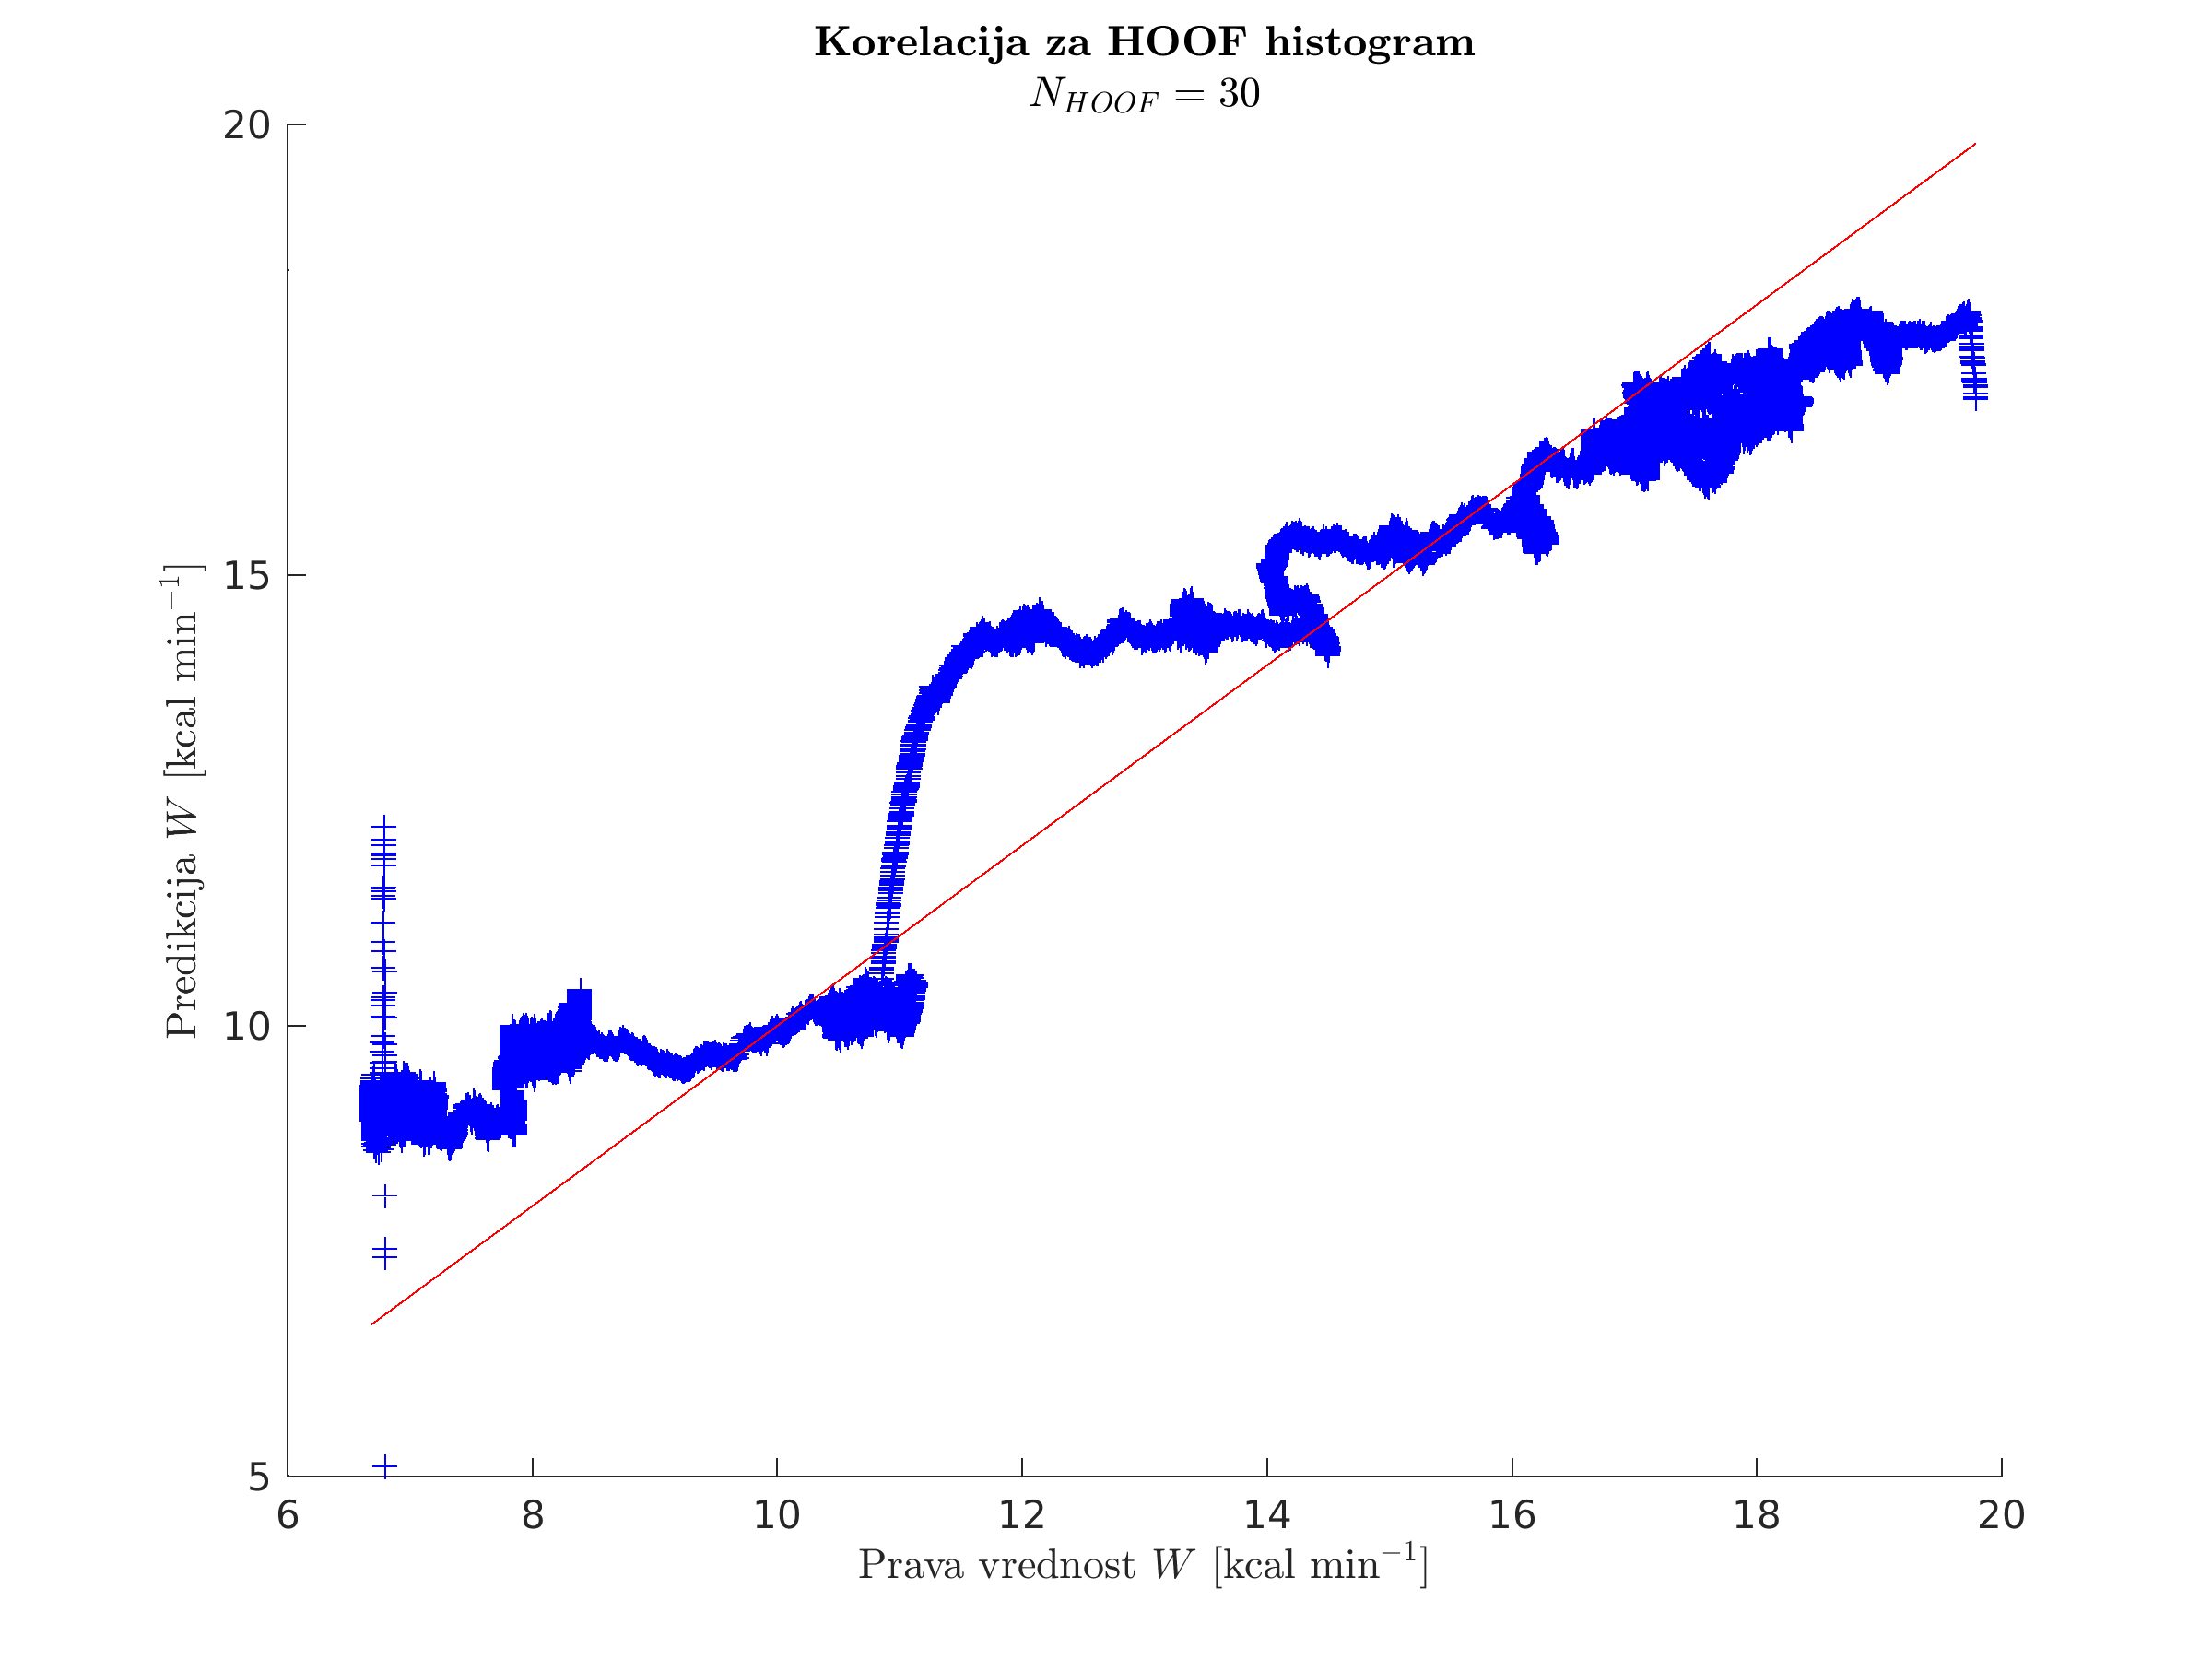
\includegraphics[width=\columnwidth]{./Slike/corr-hoof-30.png}
        \caption{Korelacija $N_{HOOF}=30$.}
        \label{fig:corr-hoof-30}
    \end{subfigure}
    ~
    \begin{subfigure}[t]{0.45\columnwidth}
      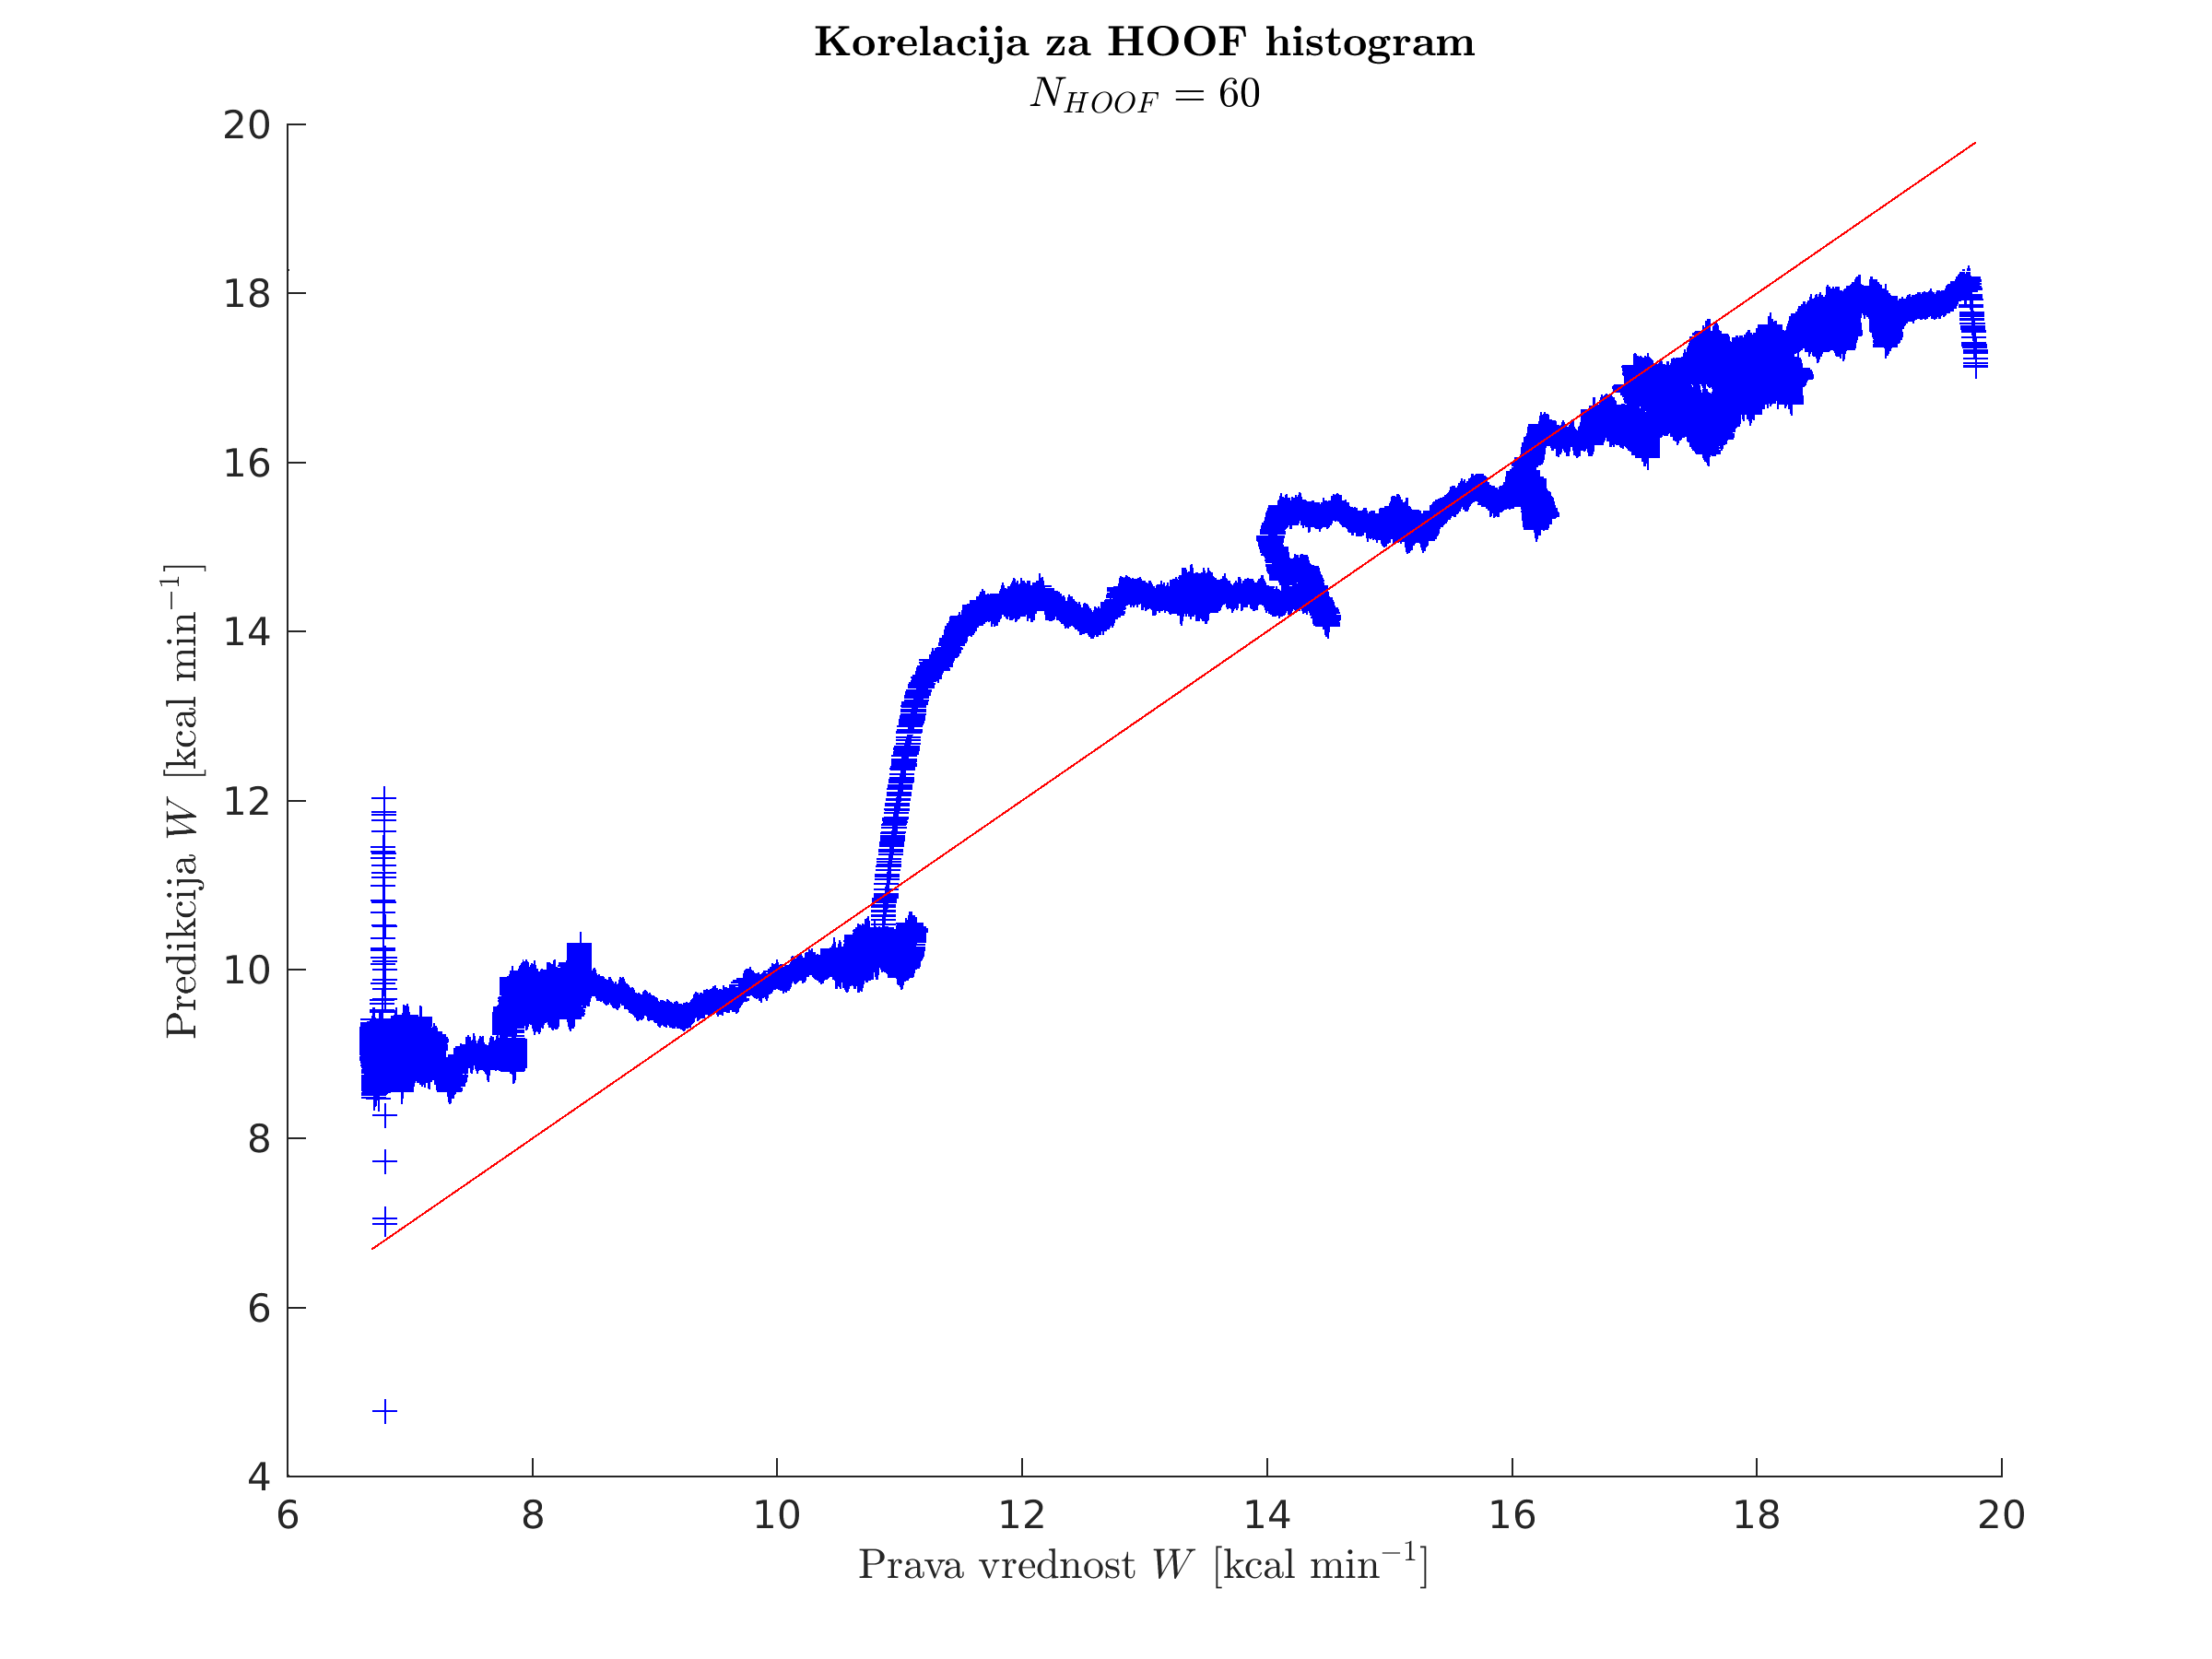
\includegraphics[width=\columnwidth]{./Slike/corr-hoof-60.png}
      \caption{Korelacija $N_{HOOF}=60$.}
      \label{fig:corr-hoof-60}
    \end{subfigure}
    ~
    \begin{subfigure}[b]{0.45\columnwidth}
      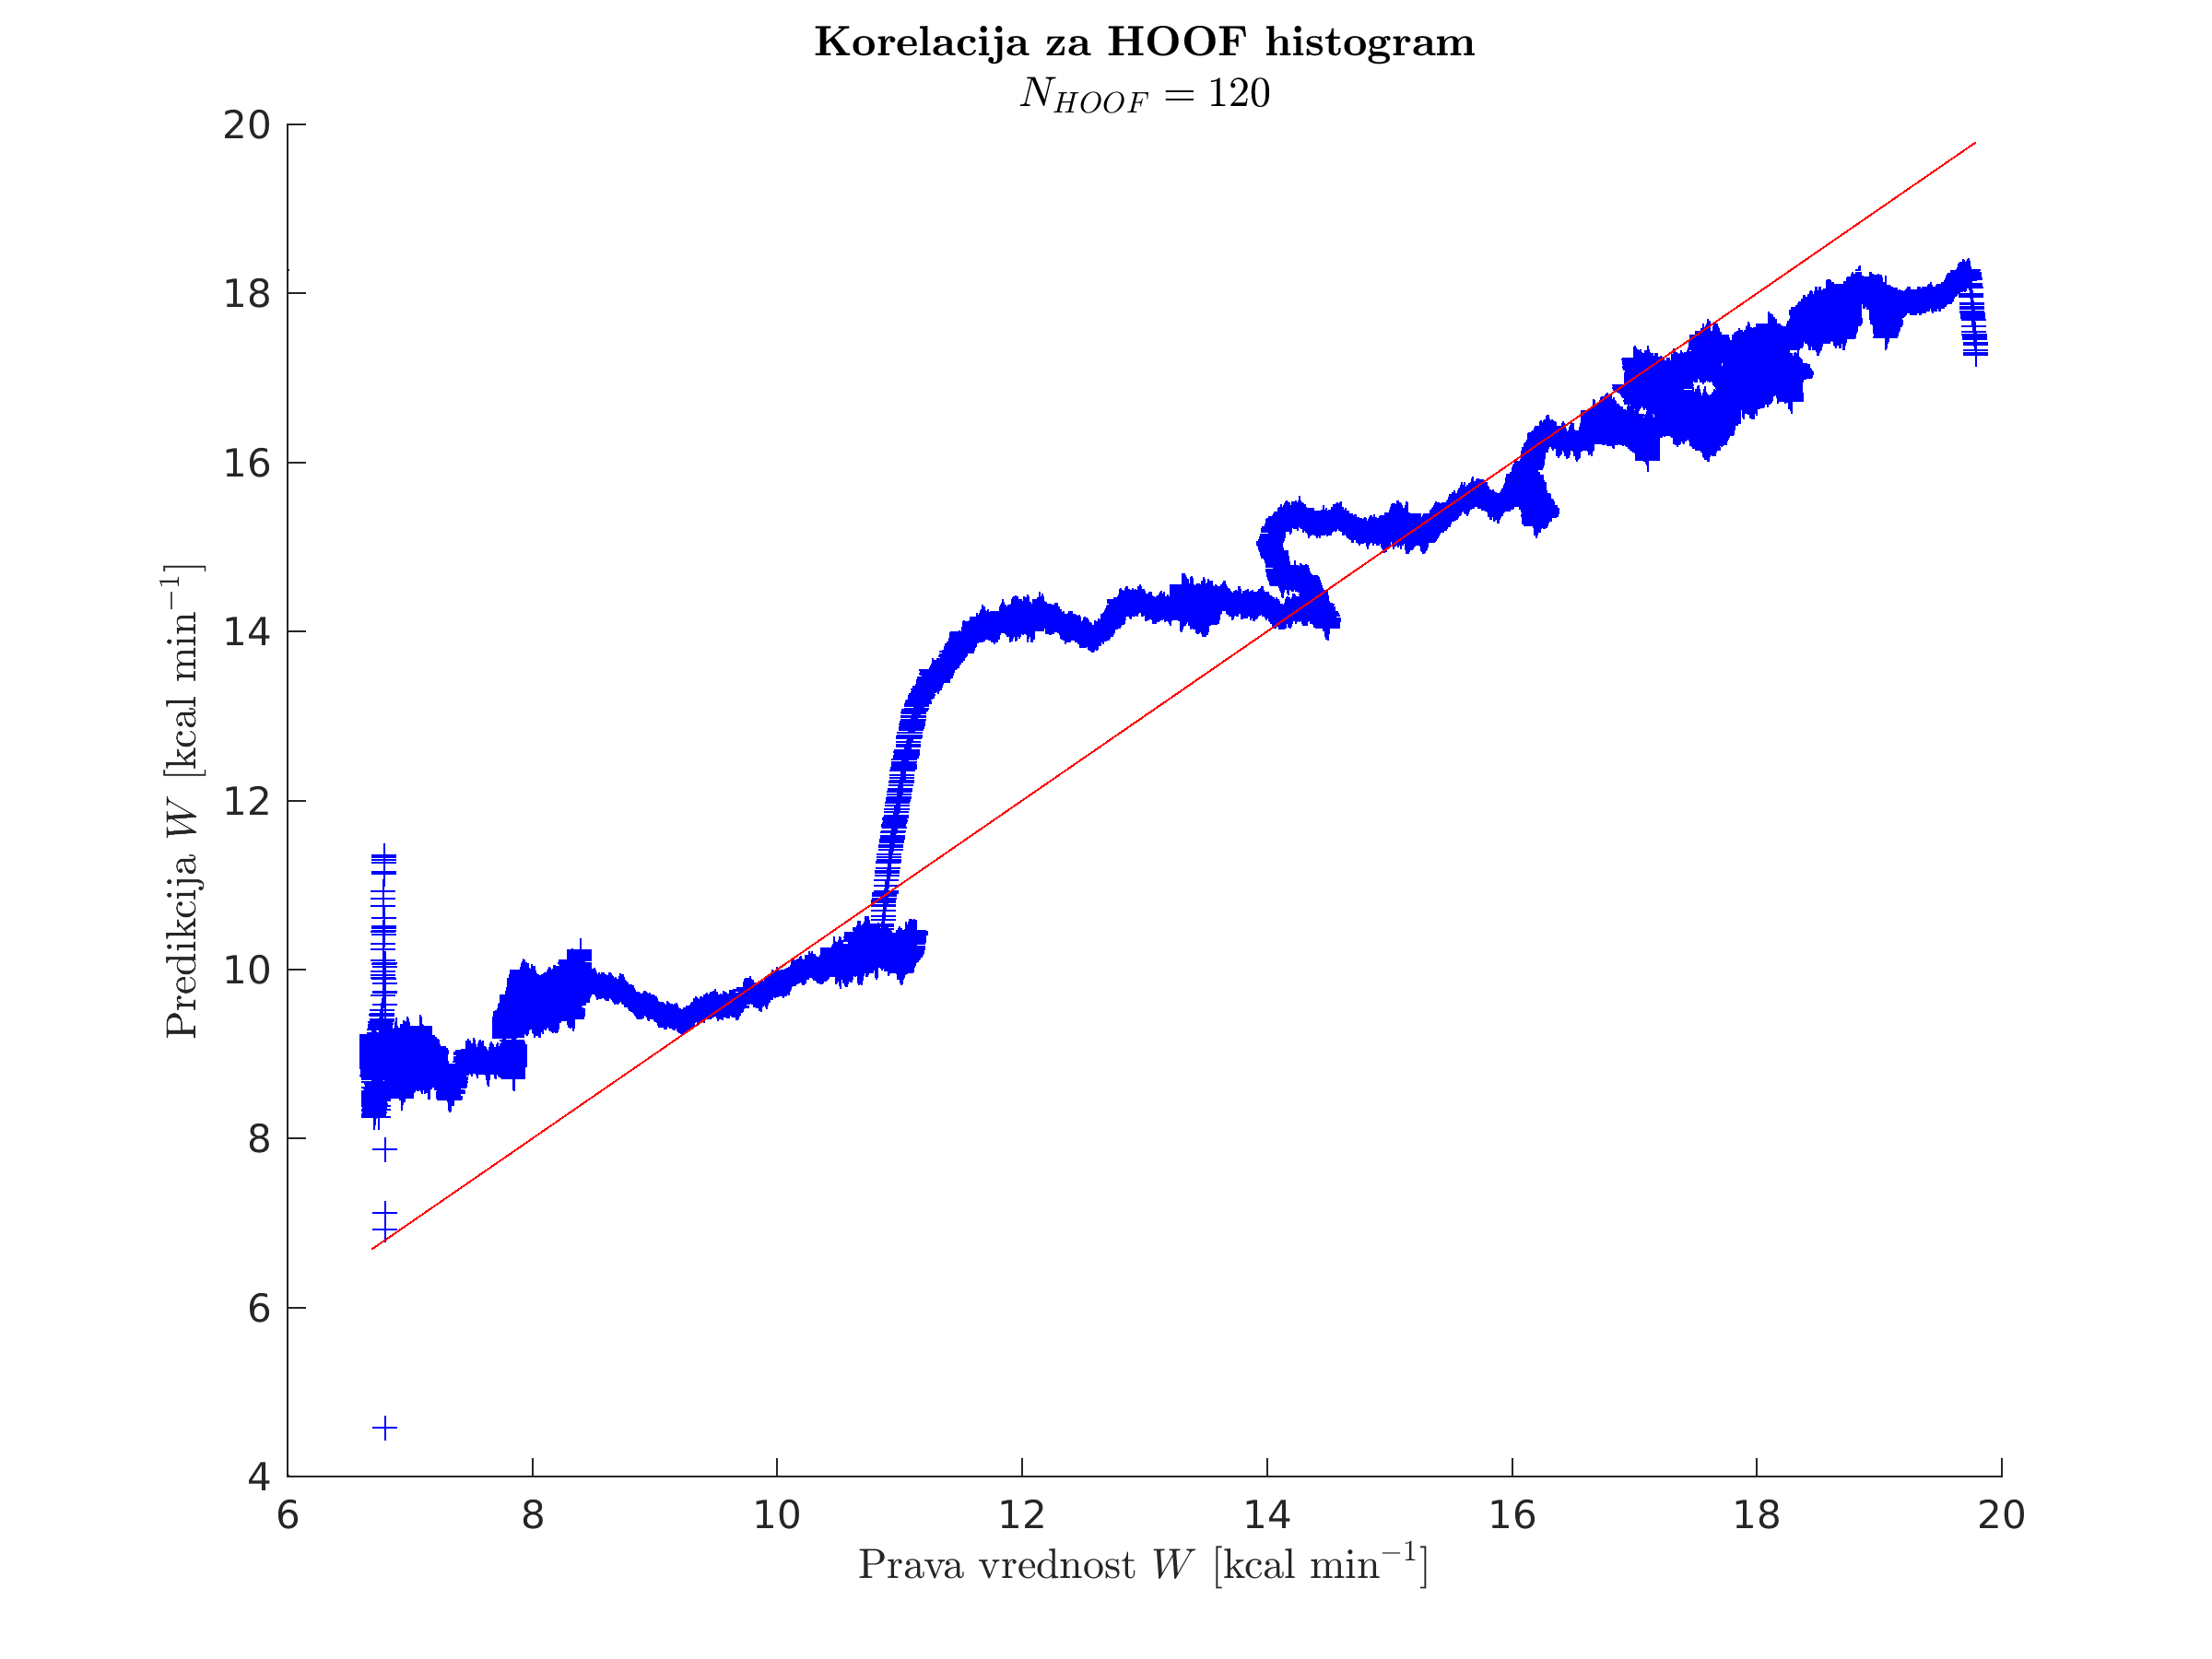
\includegraphics[width=\columnwidth]{./Slike/corr-hoof-120.png}
      \caption{Korelacija $N_{HOOF}=120$.}
      \label{fig:corr-hoof-120}
    \end{subfigure}
    ~
    \begin{subfigure}[b]{0.45\columnwidth}
      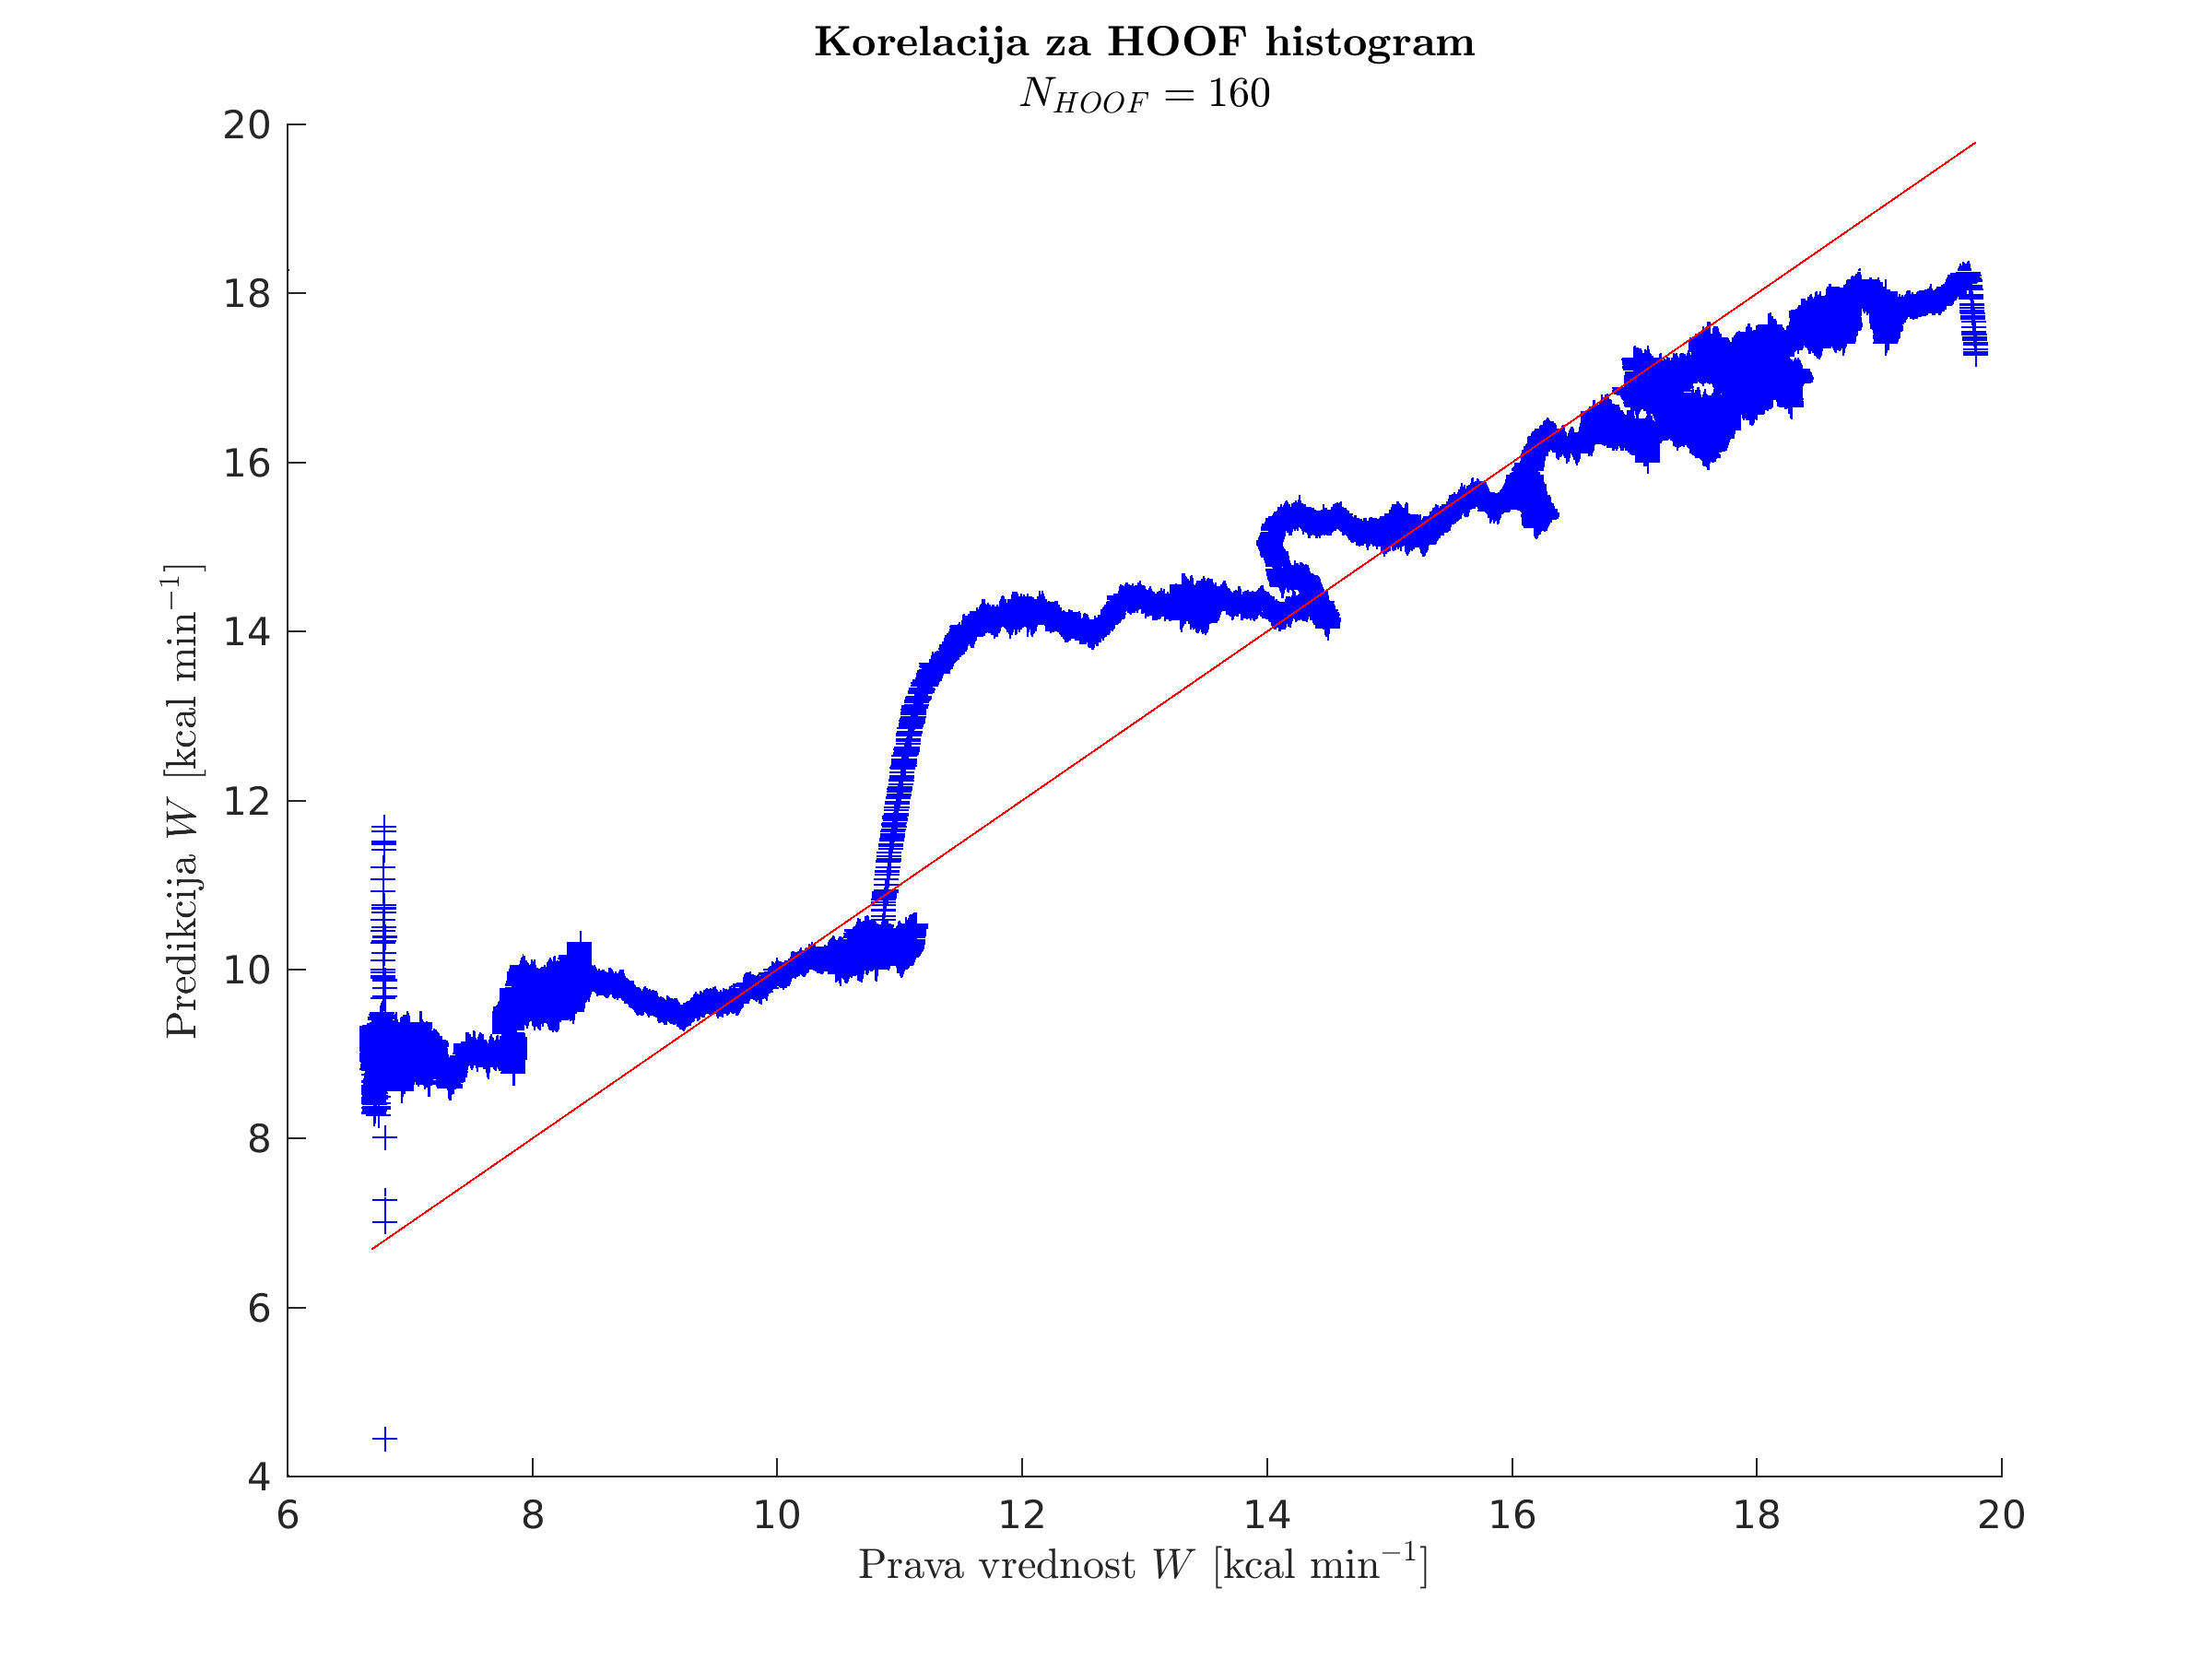
\includegraphics[width=\columnwidth]{./Slike/corr-hoof-160.png}
      \caption{Korelacija $N_{HOOF}=160$.}
      \label{fig:corr-hoof-160}
    \end{subfigure}
    \caption[Grafi korelacij modelov z različnim $N_{HOOF}$]{Grafi korelacij modelov z različnim številom stolpcev $N_{HOOF}$ HOOF deskriptorja. Rezultati so si zelo podobni.}
    \label{fig:corr-hoof}
\end{figure}





\subsection{Optimizacija HAFA deskriptorjev}
Parameter $N_{HAFA}$ smo določili na podlagi rezultatov evaluacije v tabeli \ref{tab:nhafa} in grafov korelacije med referenčnimi podatki in predikcijo \ref{fig:corr-hafa}. Za evaluacijo smo uporabili enak eksperimentalni protokol kot za HOOF značilke v poglavju \ref{sec:hoof}, s to razliko, da smo značilke normirali na intervalu $[0, 1]$ in odstranili stolpec z amplitudami $0.5$. S tem smo odstranili šum, ki se je pojavil, ko ni bilo nobenega gibanja. Amplitudo šuma smo določili, kot maksimalno vrednost amplitude, ki še ni predstavljala gibanja. Optimalni parametri evaluacijske metode so predstavljeni v tabeli \ref{tab:nhafa-param}.


\begin{table}[htb]
	\centering
    \begin{tabular}{S[table-format=2.0] S[table-format=2.3] S[table-format=1.3]  S[table-format=1.3] S[table-format=1.3]}
    \toprule
    \thead{$\mathbf{N_{HAFA}}$} & \thead{$\mathbf{C}$} & \thead{$\mathbf{\gamma}$} & \thead{$\mathbf{\epsilon}$} & \thead{MSE} \\ 
    \midrule
    30 & 8 & 5.657 & 0.616 & 4.329 \\
    60 & 8 & 5.657 & 0.616 & 4.327 \\
    120 & 8 & 5.657 & 0.616 & 4.327 \\
    160 & 8 & 5.657 & 0.616 & 4.327 \\
    \bottomrule
    \end{tabular}
    \caption[Optimalni parameteri RBF jedra modelov za določitev $N_{HAFA}$]{Optimalni parametri RBF jedra za modele z različnim številom stolpcev $N_{HAFA}$ v HAFA deskriptorju.}
    \label{tab:nhafa-param}
\end{table}

V tabeli \ref{tab:nhafa} lahko vidimo, da so rezultati praktično enaki. Za našo metodo smo izbrali $N_{HAFA}=60$, kar v grobem predstavlja $60$ različnih hitrosti z maksimalno amplitudo \SI{60}{px.f^{-1}}.

\begin{table}[htb]
	\centering
    \begin{tabular}{S[table-format=2.0] S[table-format=1.3] S[table-format=1.3] S[table-format=1.3] S[table-format=2.2]}
    \toprule
    \thead{$N_{HAFA}$} & \thead{$r$} & \thead{RAE} & \thead{RMSE} & \thead{nSV [\%]}\\
    \midrule%nSV
    30 & 0.984 & 0.213 & 0.231 & 62.08 \\%17879/28799
    \boldentry{2.0}{60} & \boldentry{1.3}{0.984} & \boldentry{1.3}{0.211} & \boldentry{1.3}{0.228} & \boldentry{2.2}{62.60} \\%18028
    120 & 0.984 & 0.211 & 0.228 & 62.63 \\%18037
    160 & 0.984 & 0.211 & 0.228 & 62.63 \\%18037
    \bottomrule
    \end{tabular}
    \caption[Rezultati evaluacije modelov z različnim $N_{HAFA}$]{Rezultati evaluacije modelov z različnim številom stolpcev $N_{HAFA}$ HAFA deskriptorja. Optimalni rezultati so odebeljeni.}
    \label{tab:nhafa}
\end{table}

\begin{figure}[htb]
	\centering
    \begin{subfigure}[t]{0.45\columnwidth}
    	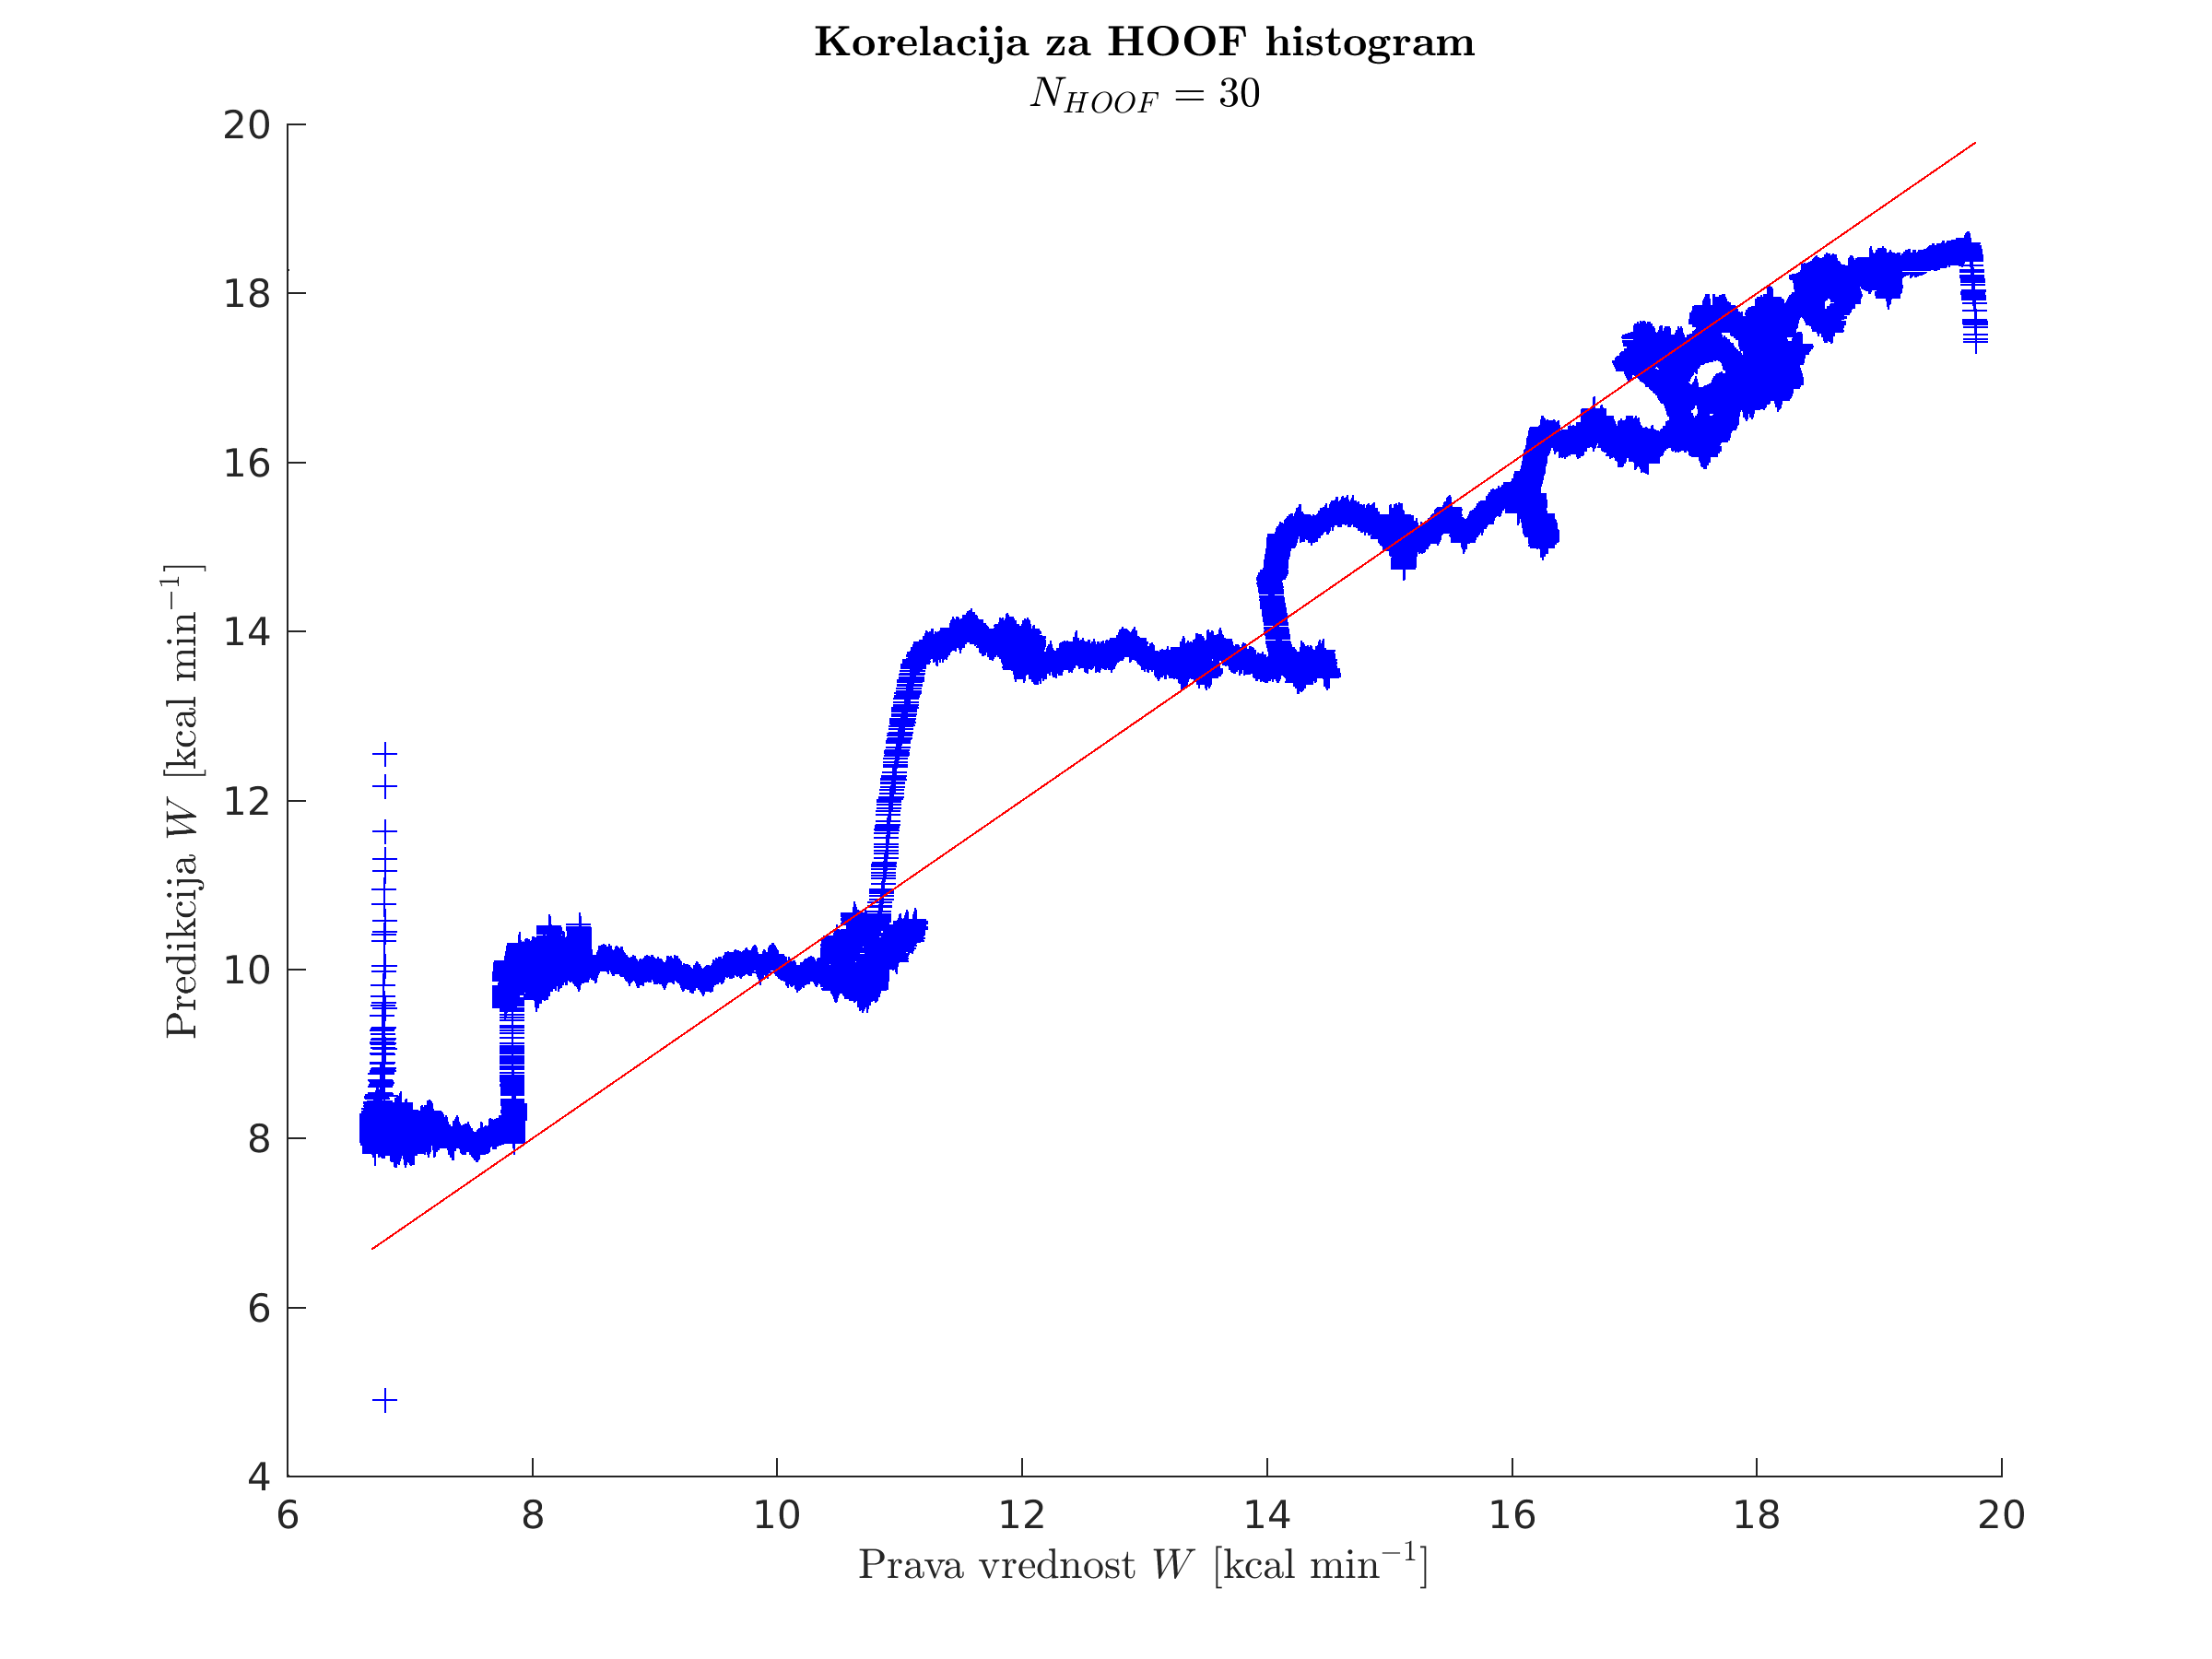
\includegraphics[width=\columnwidth]{./Slike/corr-hafa-30.png}
        \caption{Korelacija $N_{HAFA}=30$.}
        \label{fig:corr-hafa-30}
    \end{subfigure}
    ~
    \begin{subfigure}[t]{0.45\columnwidth}
      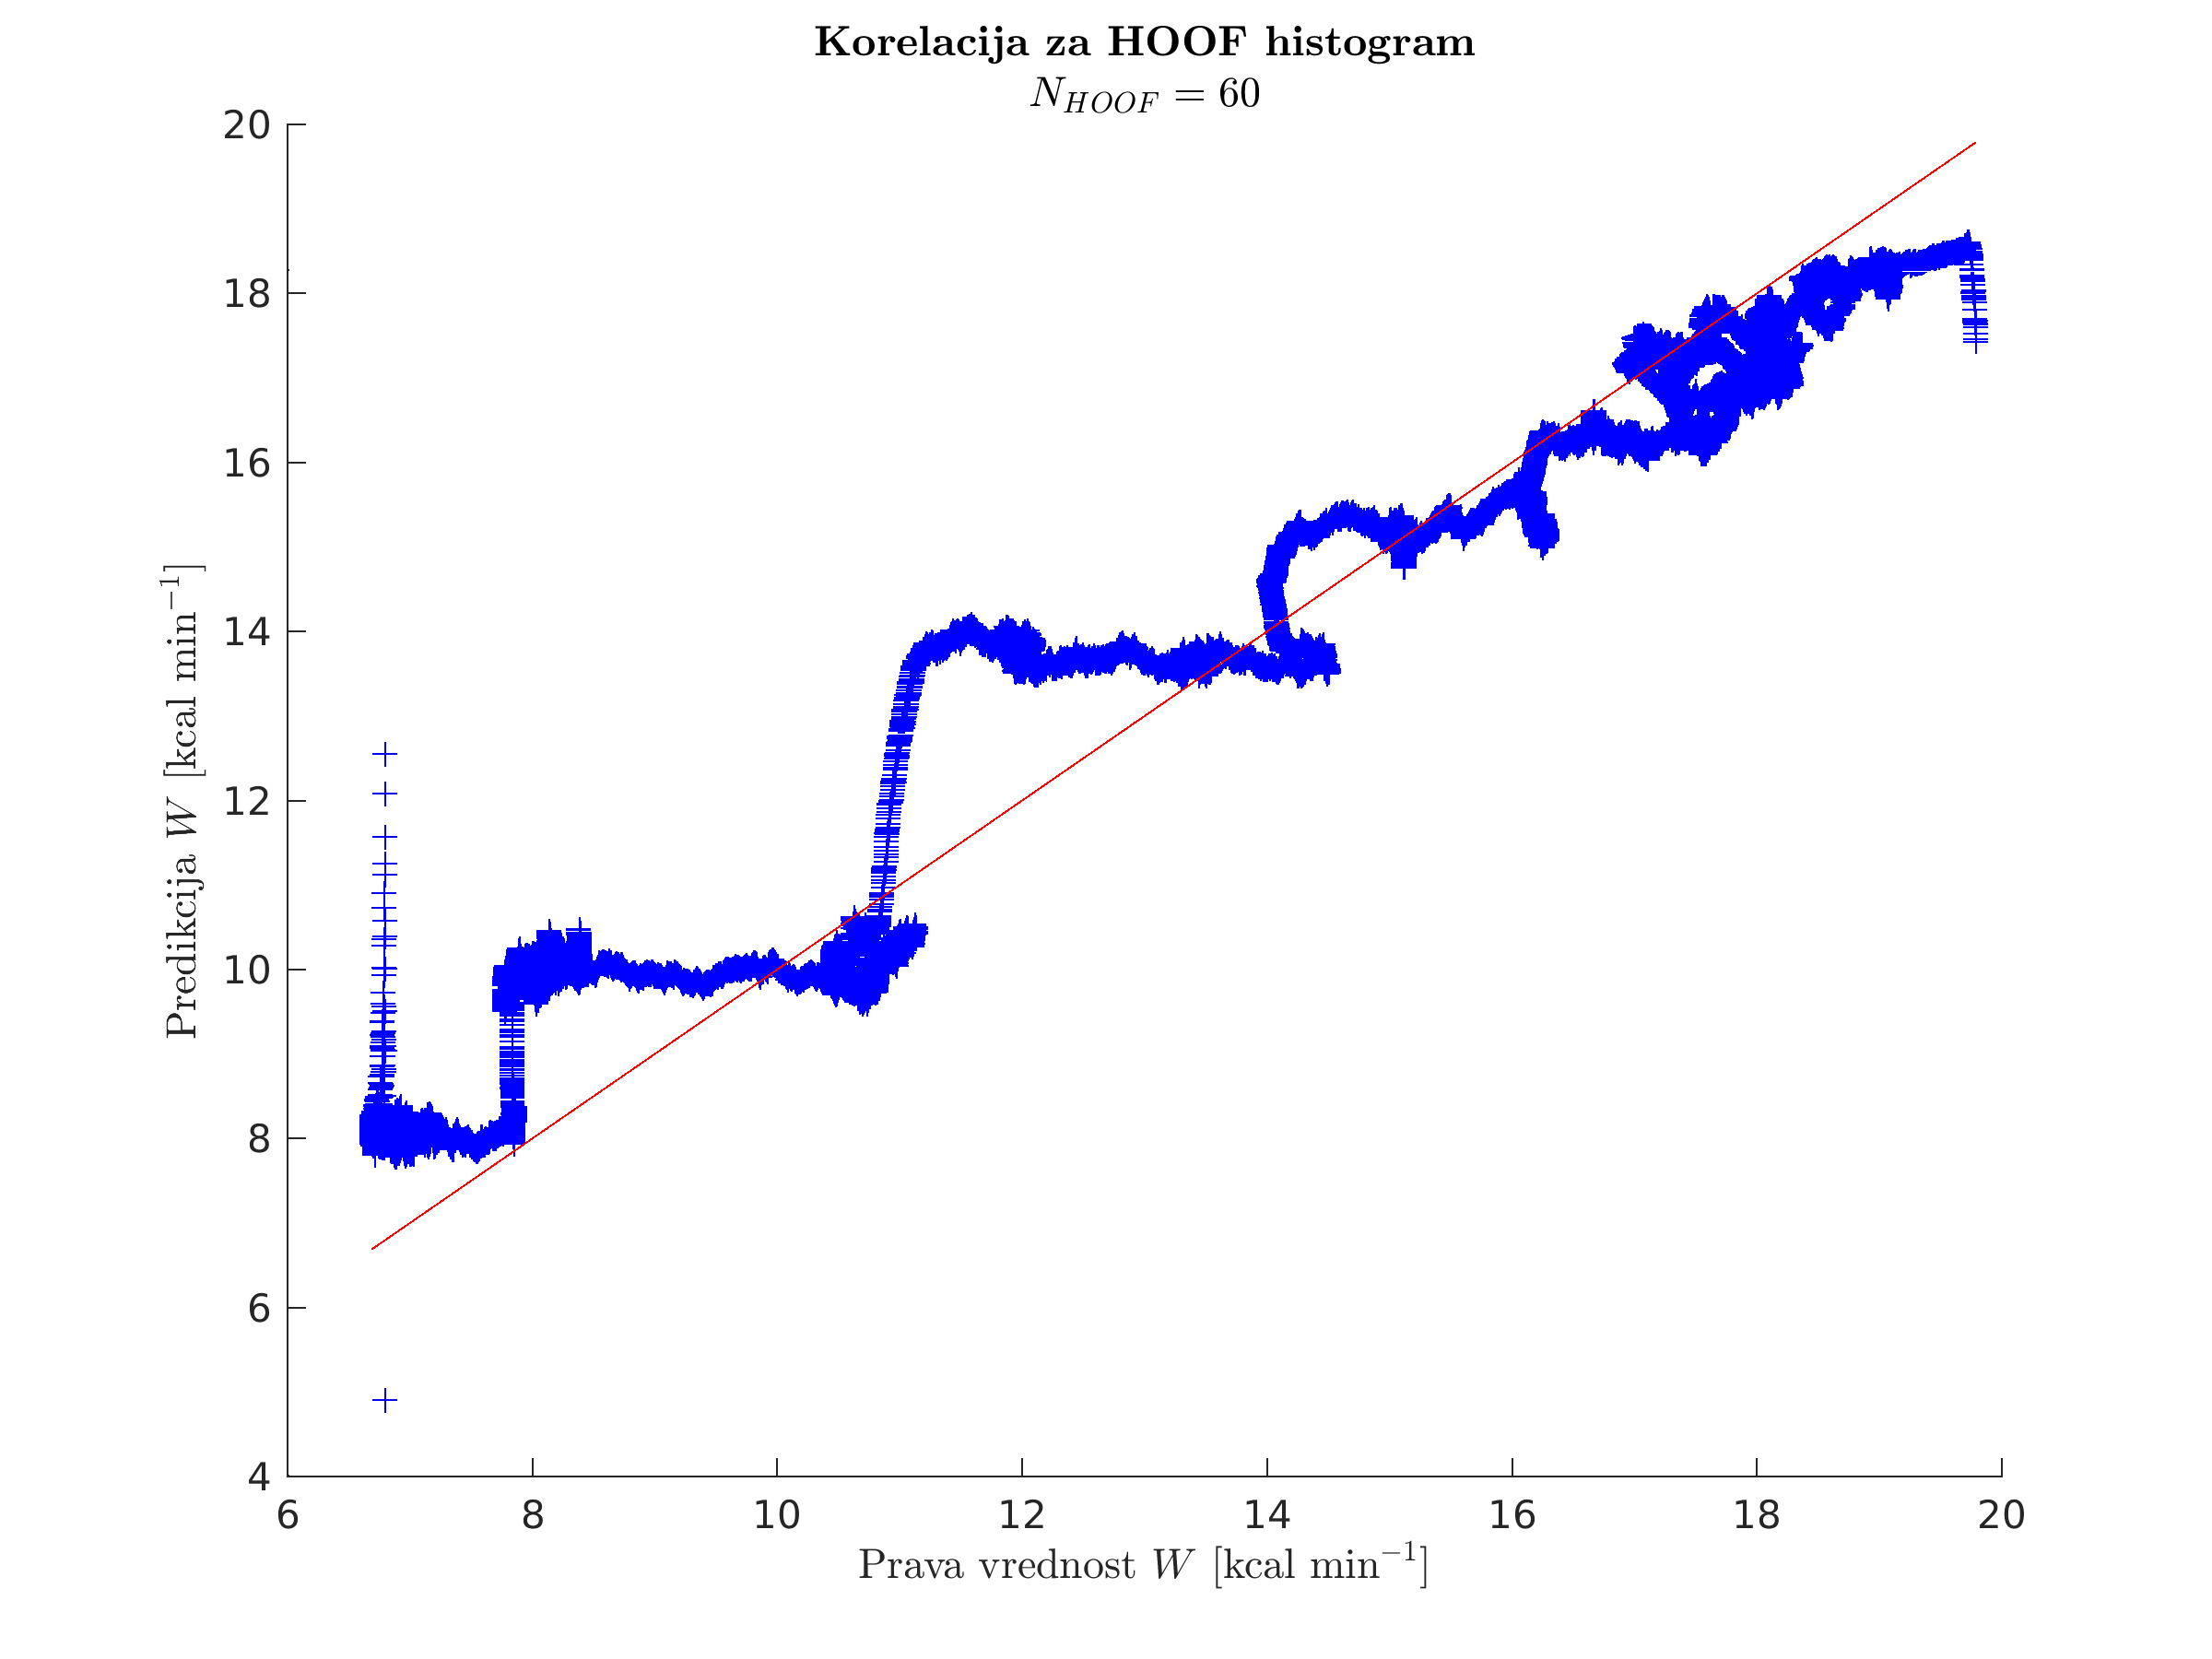
\includegraphics[width=\columnwidth]{./Slike/corr-hafa-60.png}
      \caption{Korelacija $N_{HAFA}=60$.}
      \label{fig:corr-hafa-60}
    \end{subfigure}
    ~
    \begin{subfigure}[b]{0.45\columnwidth}
      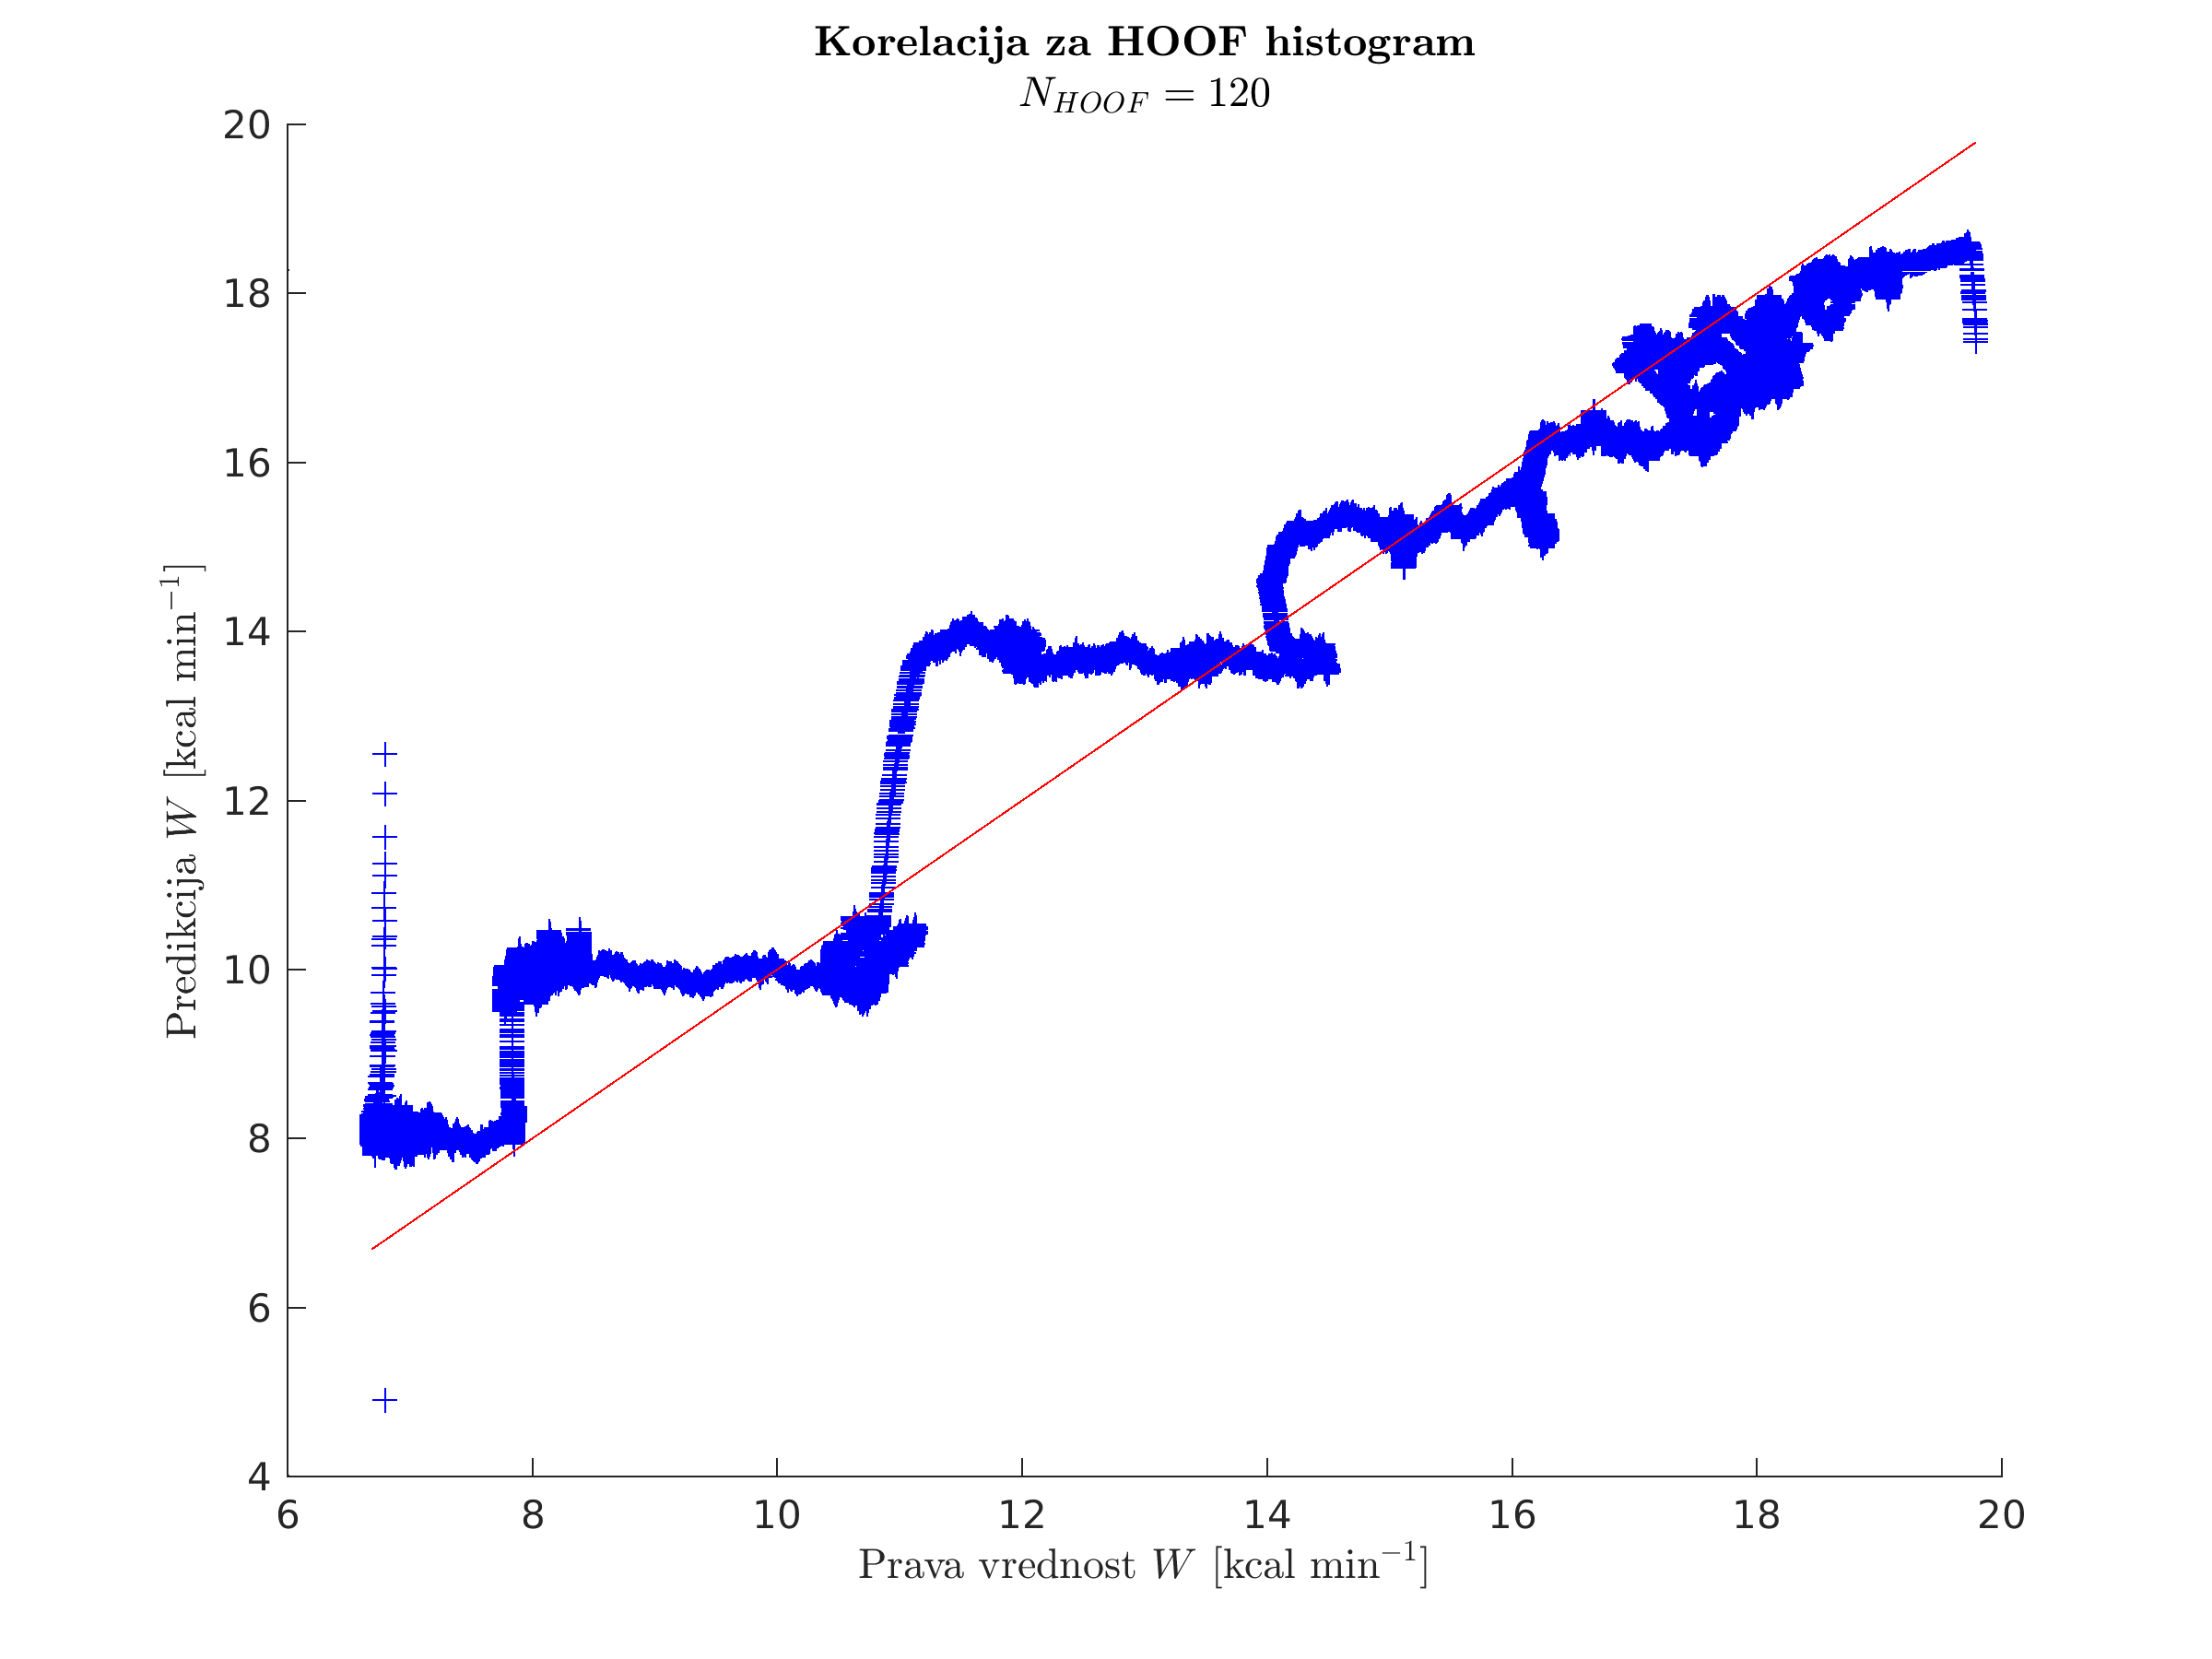
\includegraphics[width=\columnwidth]{./Slike/corr-hafa-120.png}
      \caption{Korelacija $N_{HAFA}=120$.}
      \label{fig:corr-hafa-120}
    \end{subfigure}
    ~
    \begin{subfigure}[b]{0.45\columnwidth}
      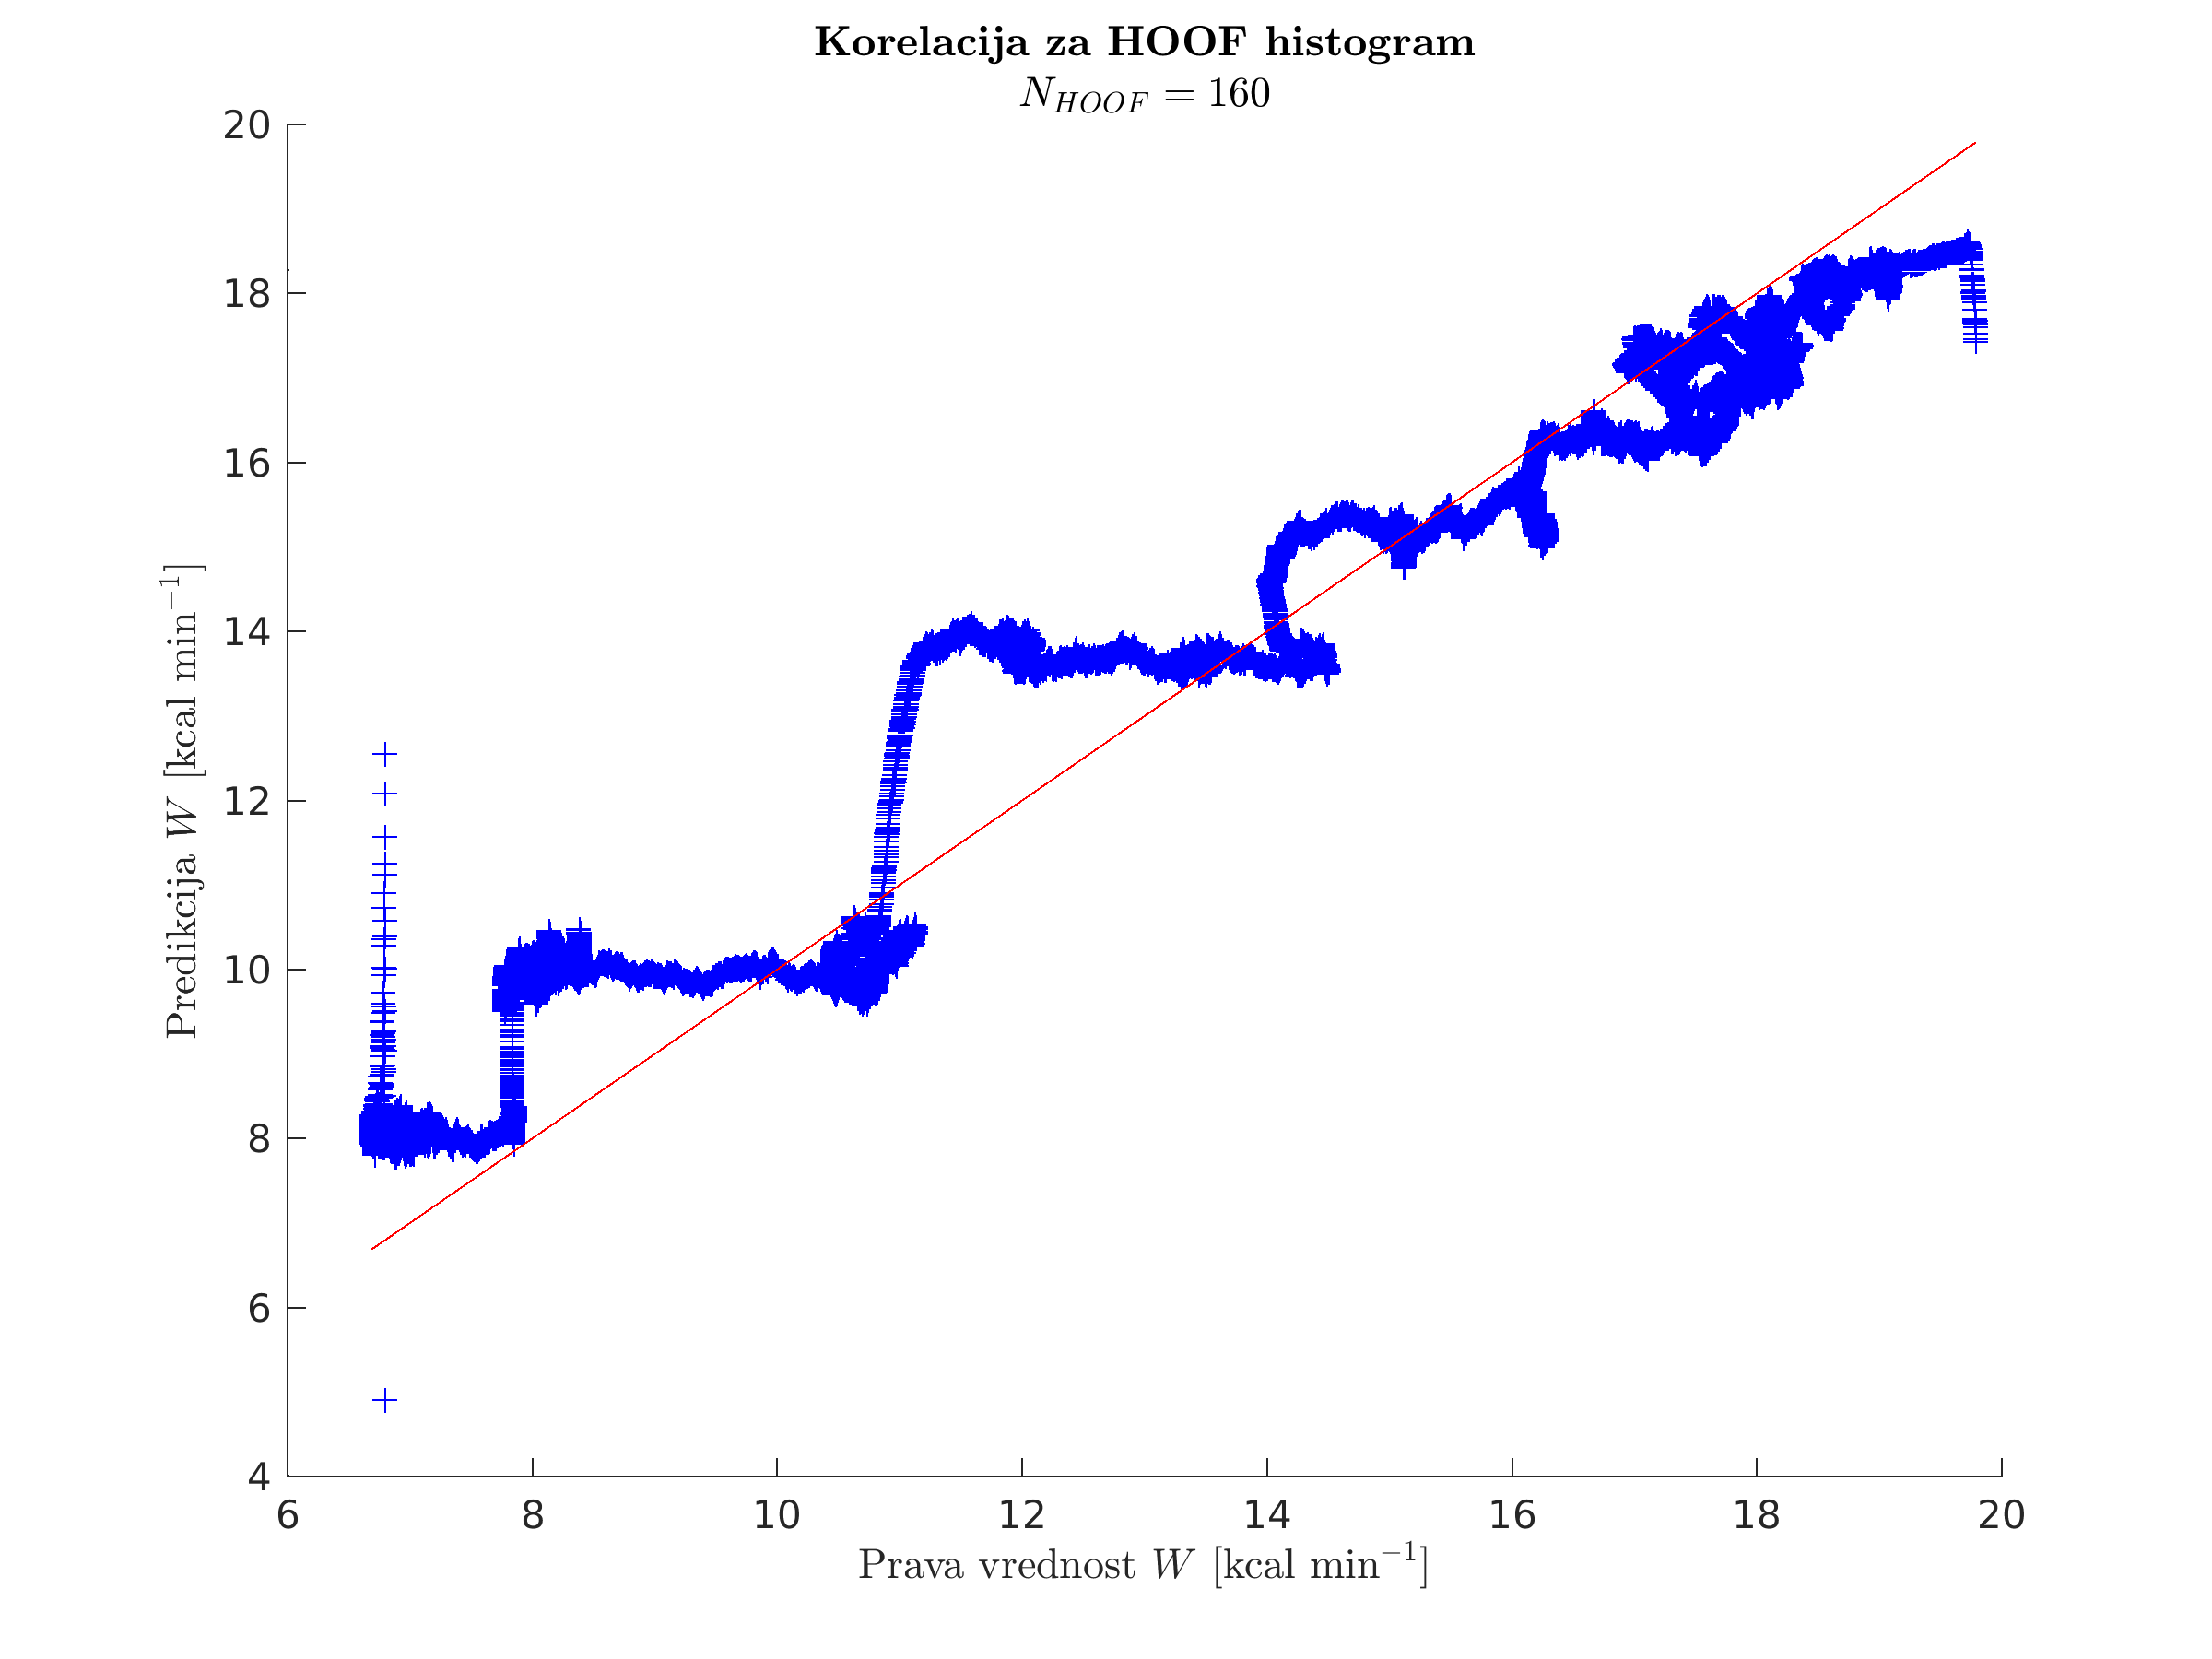
\includegraphics[width=\columnwidth]{./Slike/corr-hafa-160.png}
      \caption{Korelacija $N_{HAFA}=160$.}
      \label{fig:corr-hafa-160}
    \end{subfigure}
    \caption[Grafi korelacij modelov z različnim $N_{HAFA}$]{Grafi korelacij modelov z različnim številom stolpcev $N_{HAFA}$ HAFA deskriptorja. Rezultati so si zelo podobni.}
    \label{fig:corr-hafa}
\end{figure}



\subsection{Normalizacija HAFA deskriptorjev}
% Zakaj naj bi bila ta rešitev dobra
% teorija tovrstne kalibracije
% Kako s to kalibracijo nismo popravili stvari
% In da smo ugotovili da obstaja še prostorski tok, ki bi nam rešil težave
V praksi se pokaže, da normiran HAFA histogram ne... -> To paše pod eksperimente.




\subsection{Izbira deskriptorjev}

Chaudhry et al. \cite{chaudhry2009histograms} predlaga uporabo histogramov orientiranega optičnega toka (HOOF) za estimacijo gibanja. Vendar pa smo v preliminarnih terenskih testiranjih \cite{koporec2017observation} ugotovili, da njihova uporaba v realnih okoliščinah ni zadovoljiva. HOOF deskriptorju smo pripeli HAFA deskriptor in tako dobili razširjeni deskriptor HOOF-HAFA, ki v splošnem daje boljše rezultate, kot lahko vidimo v tabeli \ref{tab:izbira} in na primerjalnih slikah \ref{fig:izbira}.

Pri evaluaciji deskriptorjev HOOF in HOOF-HAFA smo uporabili učne vzorce hrbtne kamere terenskih testov. Evaluirali smo za podatke srčnega utripa $hr$. Srčni utrip smo za gradnjo modelov pretvorili v energijsko porabo $W$ po enačbi \eqref{eq:charlot}. Pridobljene značilke smo normirali na intervalu [0,1] in jih uporabili za učenje regresijskega modela z metodo podpornih vektorjev $\epsilon$-SVR in jedrom RBF. Za določitev optimalnih parametrov, ki so predstavljeni v tabeli \ref{tab:nhoof-param}, smo uporabili optimizacijsko metodo mrežnega iskanja \cite{hsu2003practical}. Rezultate smo filtrirali še s Gaussovim jedrom (predstavljen v \ref{sec:gaussov-filter}) velikosti $6$ in varianco $\sigma=16$. 

\begin{table}[htb]
	\centering
    \begin{tabular}{l S[table-format=2.3] S[table-format=1.3] S[table-format=1.3] S[table-format=1.3]}
    \toprule
    \thead{Deskriptor} & \thead{$\mathbf{C}$} & \thead{$\mathbf{\gamma}$} & \thead{$\mathbf{\epsilon}$} & \thead{MSE} \\ 
    \midrule
    HOOF & 2.828 & 11.314 & 0.435 & 2.192 \\
    HOOF-HAFA & 5.657 & 2.828 & 0.154 & 1.781 \\
    \bottomrule
    \end{tabular}
    \caption[Optimalni parameteri RBF jedra modelov za izbiro deskriptorjev]{Optimalni parametri RBF jedra za modele z različnim deskriptorjem.}
    \label{tab:izbira-param}
\end{table}


\begin{table}[htb]
	\centering
    \begin{tabular}{l S[table-format=1.3] S[table-format=1.3] S[table-format=1.3] S[table-format=2.2]}
    \toprule
    \thead{Deskriptor} & \thead{$r$} & \thead{RAE} & \thead{RMSE} & \thead{nSV [\%]}\\
    \midrule%nSV
    HOOF & 0.992 & 0.336 & 0.317 & \boldentry{2.2}{82.34} \\%2187/2656
    \textbf{HOOF-HAFA} & \boldentry{1.3}{0.991} & \boldentry{1.3}{0.157} & \boldentry{1.3}{0.205} & 89.53 \\%2378
    \bottomrule
    \end{tabular}
    \caption[Rezultati evaluacije modelov z različnim deskriptorjem]{Rezultati evaluacije modelov z različnim deskriptorjem. Optimalni rezultati so odebeljeni. Vidimo lahko, da se bolje odnese razširjeni deskriptor HOOF-HAFA, čeprav model uporablja več podpornih vektorjev. }
    \label{tab:izbira}
\end{table}



\begin{figure}[htb]
	\centering
    \begin{subfigure}[t]{0.45\columnwidth}
      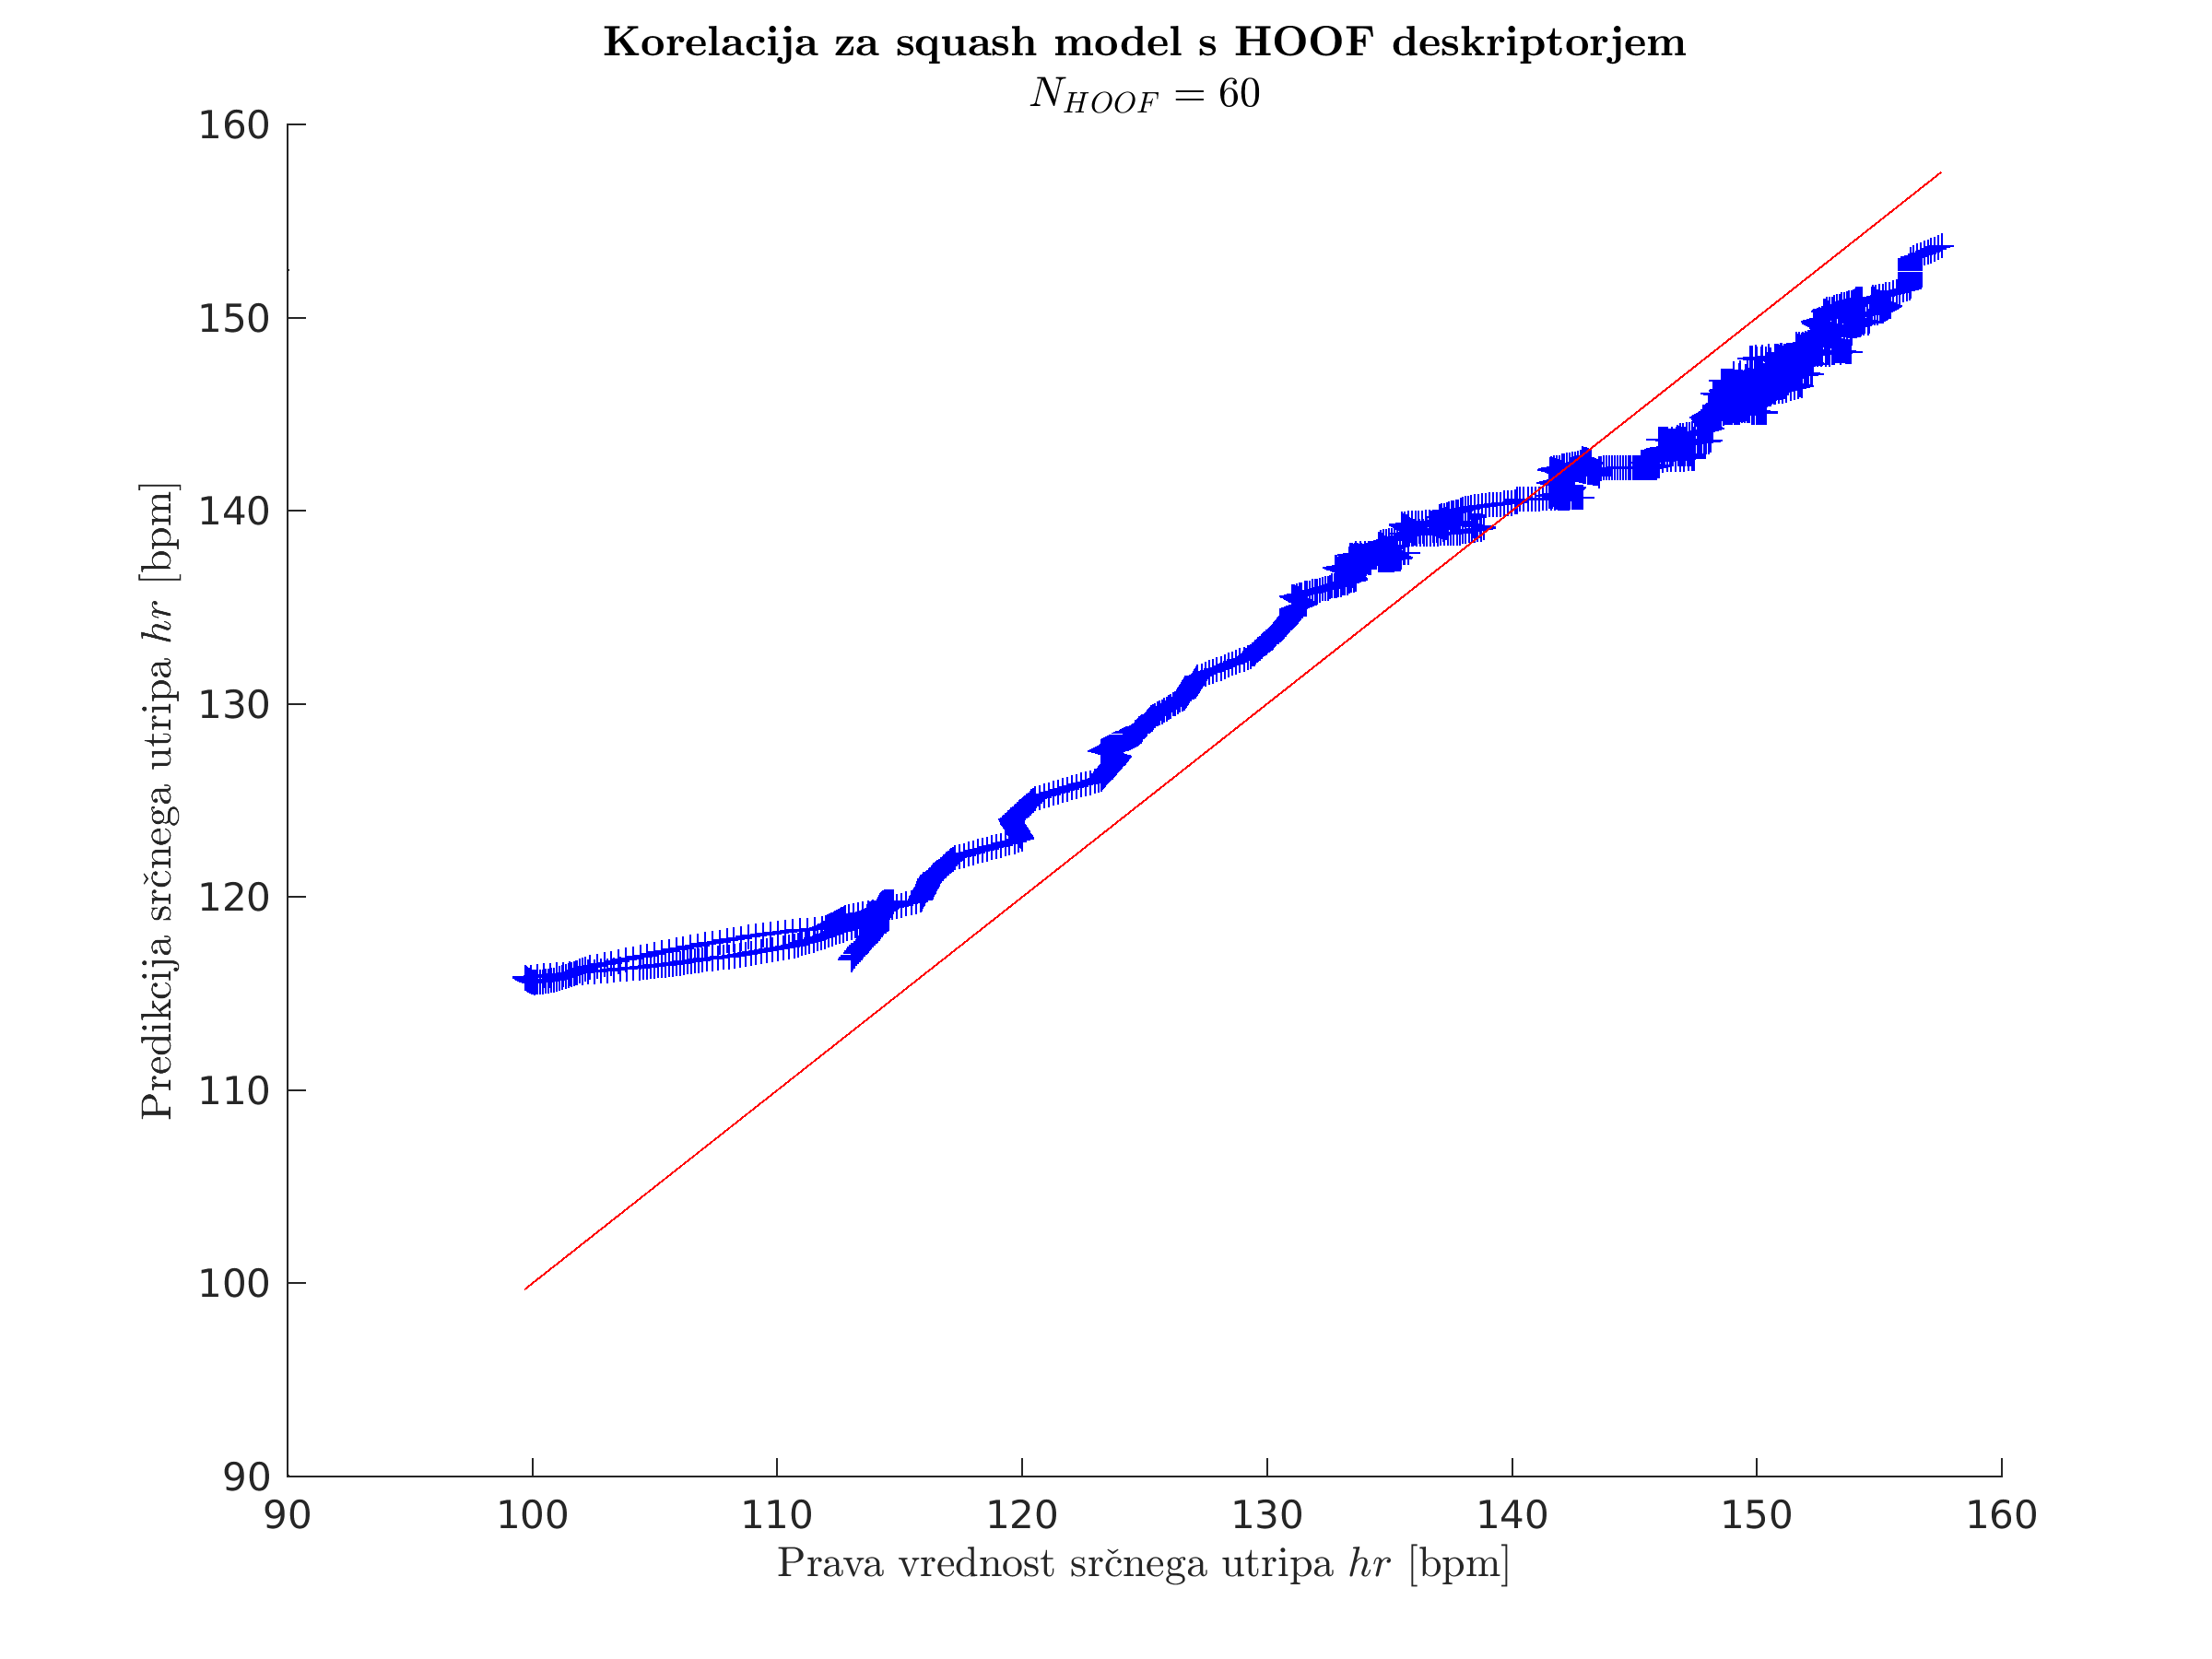
\includegraphics[width=\columnwidth]{./Slike/corr-hoof.png}
      \caption{Korelacija $N_{HOOF}=60$.}
      \label{fig:izbira-hoof}
    \end{subfigure}
    ~
    \begin{subfigure}[t]{0.45\columnwidth}
      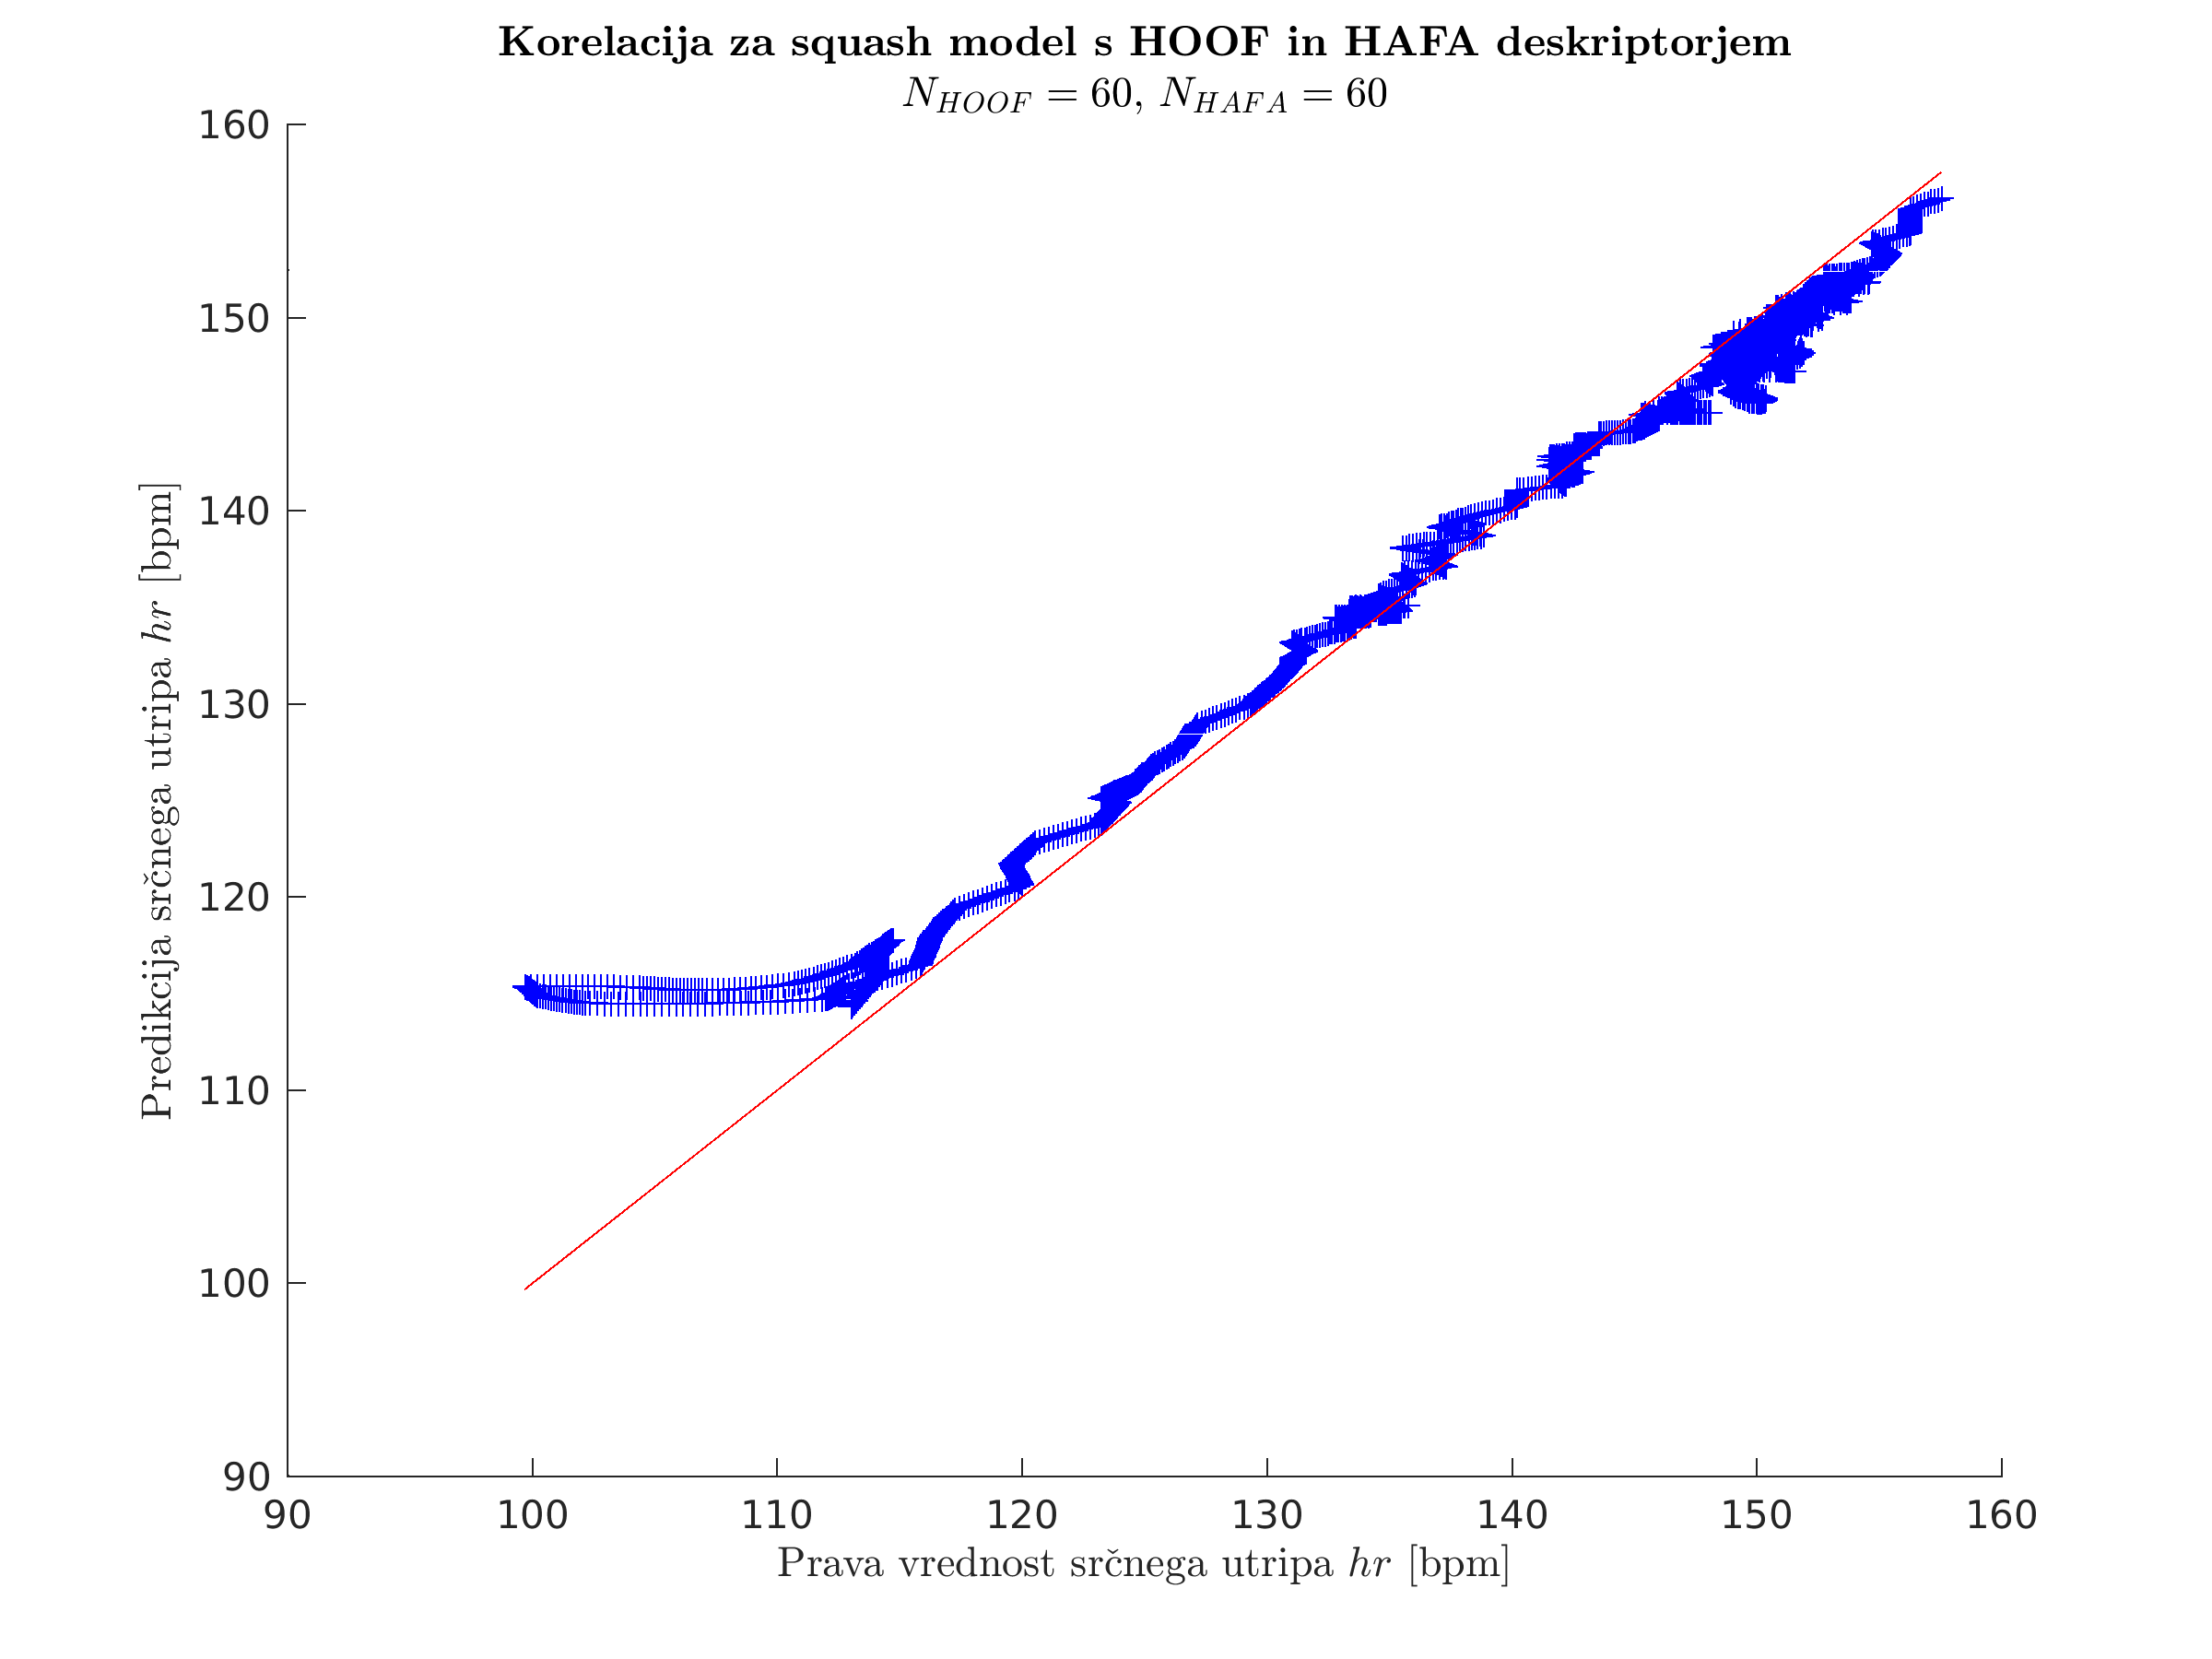
\includegraphics[width=\columnwidth]{./Slike/corr-hoof-hafa.png}
      \caption{Korelacija $N_{HOOF}=60$,\\$N_{HAFA}=60$.}
      \label{fig:izbira-hoofhafa}
    \end{subfigure}
    \caption[Primerjava modelov s HOOF in HOOF-HAFA deskriptorji]{Primerjava grafov korelacij modelov z različnimi deskriptorji. Model \subref{fig:izbira-hoof}) smo naučili s HOOF deskriptorjem. Model \subref{fig:izbira-hoofhafa}) smo naučili s HOOF in HAFA deskriptorjem. Posamezen vzorec je tako vseboval $120$ značilk. Pri primerjavi korelacije lahko opazimo vidno razliko. Model \subref{fig:izbira-hoofhafa}) dokazuje, da je razširjeni deskriptor boljši.}
    \label{fig:izbira}
\end{figure}





\subsubsection{Regresija \texorpdfstring{$\nu$}{nu}-RBF}





\subsection{Optični tok}
Na podlagi opisanih lastnosti metod optičnega toka v poglavju \ref{sec:metode-of} smo se odločili, da bomo v tem delu uporabili diferencialno metodo. Kljub višji računski zahtevnosti, ki ob današnji tehnologiji ne predstavlja več takega problema, smo želeli računati gost optični tok. Z gostim optičnim tokom tako dobimo natačno aproksimacijo polja gibanja za celotno telo. Prav tako nimamo problemov pri estimaciji energijske porabe za hitre gibe, kot bi bilo to v primeru uporabe ujemlanih metod. Ker je glavni namen uporaba in ne implementacija diferencialne metode, smo se osredotočili na Farneb{\"a}ck algoritem, ki je dostopen v knjižnici OpenCV.


\subsection{Prostorski tok}
Ker smo v našem delu za računanje prostorskega toka uporabili Kinect senzorje, smo potrebovali metodo, ki temelji na RGB-D podatkih. Ker je glavni namen uporaba in ne implementacija algoritma prostorskega toka, smo se osredotočili na PD-Flow algoritem, ki je javno dostopen \cite{jaimez2015primal}. Algoritem je podrobneje opisan v poglavju \ref{sec:pd-flow}.





\subsection{Sledilniki}
\subsubsection{Način izbire sledilnikov}\label{sec:pogoji-sledilnikov}
Pri izbiri sledilnikov smo se osredotočili na pogoje, ki jim morajo sledilniki v največji meri zadostiti.

\paragraph{Način sledenja.} Sledilnik mora dobro slediti osebam, ostali objekti niso pomembni. Sledenje mora biti zanesljivo, saj je od njega odvisna merilna napaka. Pri tem moramo upoštevati delovanje tudi v primerih, kadar tarča izgine iz slike. Sledenje mora delovati čimdaljši čas tako, da ne potrebujemo ponovne inicializacije. Inicializacijo sledilnika moramo opraviti samo na prvi sliki zaporedja, kar pomeni, da mora sledilnik vsebovati indirektno učenje (angl. offline training).

\paragraph{Implementacija.} Zaradi uporabe sledilnika v merilnem instrumentu, mora ta delovati v realnem času oziroma čim hitreje. Ker namen tega dela ni implementacija sledilnika, mora biti ta implementiran v prosto dostopni izvorni kodi. 


\subsection{Sledilnik za optični tok}
Na podlagi že prej opisanih pogojev, smo za merilno metodo z optičnim tokom našli sledilnik TLD avtorja Kalal et. al \cite{kalal2012tracking}. Prosto dostopne so tri implementacije sledilnika in sicer v knjižnici ccv (CCV-TLD), v knjižnici OpenCV (OPENCV-TLD) in c++ izvorna koda (NEBEHAY-TLD). Implementaciji iz knjižnic ccv in OpenCV se nekoliko razlikujeta od izvirnega dela \cite{kalal2012tracking}, NEBEHAY-TLD pa je samo prepis matlabove izvorne kode. Ker ni nobena implementacija zadovoljivo delovala na testnih squash posnetkih, smo poskusili še sledilnikom KCF \cite{danelljan2014adaptive} in CORR \cite{danelljan2014accurate}. KCF je implementiran v knjižnici OpenCV, CORR pa v knjižnici Dlib \cite{king2009dlib}. 




\subsubsection{Testiranje sledilnikov}
Sledilnike smo testirali na sekvencah slik \textit{handball1} in \textit{handball2} podatkovne baze VOT2016 \cite{kristan2016visual}. Sledila je še hitra vizualna ocena delovanja na kratkih izsekih video posnetka \cite{squashtv2014squash}.

Pri testiranju sekvenc slik podatkovne baze VOT2016 smo poenostavili rotirajoča referenčna področja detekcij na nerotirajoča področja. Pri tem smo za zgornji levi kot $T_0(x,y)$ in spodnji desni kot $T_1(x,y)$ uporabili enačbo \eqref{eq:vot-bb}, kjer so $\left( x_i, y_i\right), \forall i=1,\ldots,4$ ogljišča rotirajočega referenčnega področja. 

\begin{equation}
\begin{aligned}
	T_0(x,y) &= \left( \min_{i = 1,\ldots,4}\left\{x_i \right\}, 
    \min_{i=1,\ldots,4}\{y_i \} \right) \\
    T_1(x,y) &= \left( \max_{i = 1,\ldots,4}\left\{x_i \right\}, 
    \max_{i=1,\ldots,4}\{y_i \} \right)
\end{aligned}
\label{eq:vot-bb}
\end{equation}

Ker je za naš sledilnik najbolj pomembno zanesljivo delovanje, smo izbrali preprosto mero prekrivanja področja \eqref{eq:region-overlap}, ki je navedena tudi v \cite{vcehovin2016visual}. $\Lambda$ predstavlja opis tarče, $R_t$ je področje tarče ob času $t$, $N$ je število slik v zaporedju, $G$ predstavlja referenco in $T$ tarčo. S prekrivanjem področja dobimo rezultate na intervalu $\left[0,1\right]$. Večje število predstavlja boljši rezultat.

\begin{align}
	\Lambda &= \left\{R_t\right\}^N_{t=1}, \nonumber \\
	\Phi(\Lambda^G, \Lambda^T) &= \left\{\phi_t\right\}^N_{t=1}, \nonumber \\
    \phi_t &= \frac{R_t^G \cap R_t^T }{R_t^G \cup R_t^T} \label{eq:region-overlap}
\end{align}


Video posnetek \cite{squashtv2014squash} smo za potrebe vizualne ocene delovanja na squash posnetkih razdelili na več kratkih izsekov. Pri tem smo uporabili le hrbtne posnetke mirujoče kamere. 

Rezultati testiranja so prikazani v tabeli \ref{tab:region-overlap}. Za izbrane sledilnike smo določili povprečje prekrivanja področja za posamezen posnetek. V tretjem stolpcu je predstavljeno povprečje prekrivanja glede na oba posnetka. Najboljši rezultati so odebeljeni. Po tabeli \ref{tab:region-overlap} se za posnetek \textit{handball1} najbolje izkaže CORR sledilnik. Za posnetek \textit{handball2} smo dobili najboljše rezultate pri sledilniku OPENCV-TLD. V povprečju se najbolje izkaže sledilnik CORR.




\begin{table}[htb]
	\centering
    \begin{tabular}{l S[table-format=1.3] S[table-format=1.3] S[table-format=1.3]}
    \toprule
    \thead{Sledilnik} & \thead{handball1} & \thead{handball2} & \thead{Povprečje}  \\
    \midrule%nSV
    NEBEHAY-TLD & 0.035 & 0.130 & 0.083 \\
    CCV-TLD & 0.117 & 0 & 0.117 \\
    OPENCV-TLD & 0.002 & \boldentry{1.3}{0.178} & 0.09 \\
    CORR & \boldentry{1.3}{0.214} & 0.160 & \boldentry{1.3}{0.187} \\
    \textbf{KCF} & {0.161} & {0.166} & {0.164} \\
    \bottomrule
    \end{tabular}
    \caption[Povprečje prekrivanja področja za posamezen sledilnik]{Povprečje prekrivanja področja za posamezen sledilnik in posnetek. V tretjem stolpcu je predstavljeno povprečje prekrivanja glede na oba posnetka. Najboljši rezultati so odebeljeni. Po tabeli \ref{tab:region-overlap} se za posnetek \textit{handball1} najbolje izkaže CORR sledilnik. Za posnetek \textit{handball2} smo dobili najboljše rezultate pri sledilniku OPENCV-TLD. V povprečju se najbolje izkaže sledilnik CORR.}
    \label{tab:region-overlap}
\end{table}


Na sliki \ref{fig:tracker-visual} lahko vidimo primer delovanja sledilnikov za oba posnetka. Referenčni igralec, ki mu morajo slediti ima rumeno majico. Za posnetek \textit{handball1} je predstavljena 15. slika, za posnetek \textit{handball2} pa 111. slika. Rezultati v tabeli \ref{tab:region-overlap} se skladajo z opažanji na sliki \ref{fig:tracker-visual}.

\begin{figure}[htb]
\centering

	\begin{subfigure}[t]{0.45\columnwidth}
      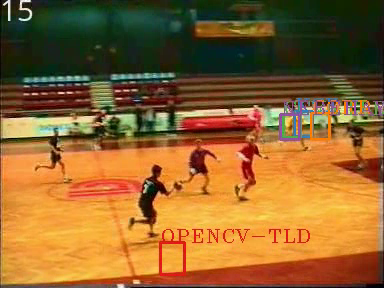
\includegraphics[width=\columnwidth]{./Slike/handball1-example.png}
      \caption{15. slika posnetka \textit{handball1}.}
      \label{fig:handball1}
    \end{subfigure}
    ~
    \begin{subfigure}[t]{0.45\columnwidth}
      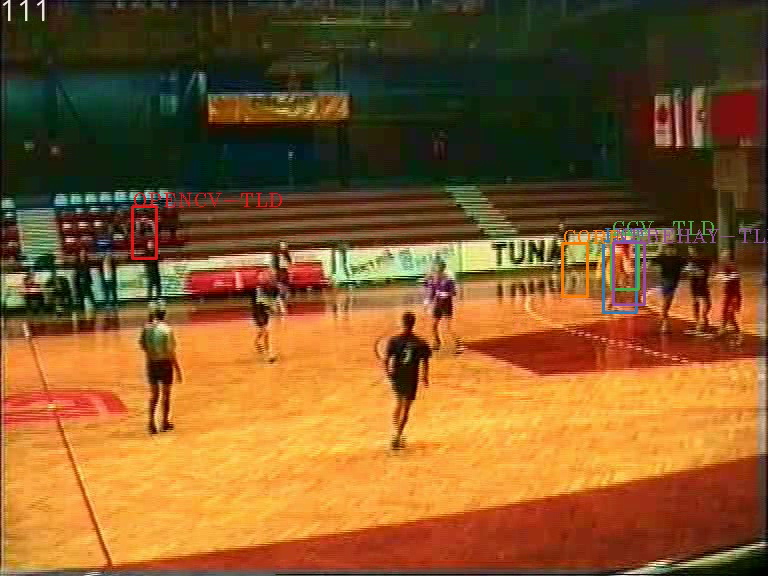
\includegraphics[width=\columnwidth]{./Slike/handball2-example.png}
      \caption{111. slika posnetka \textit{handball2}.}
      \label{fig:handball2}
    \end{subfigure}  
\caption[Primer delovanja sledilnikov za \textit{handball} posnetke]{Primer delovanja sledilnikov za \textit{handball} posnetke. Referenčni igralec, ki mu morajo slediti ima rumeno majico. }
\label{fig:tracker-visual}
\end{figure}




Čeprav smo z mero določili, da se je najbolje izkazal sledilnik CORR, se je pri hitri vizualni oceni sledenja na izsekih posnetka \cite{squashtv2014squash} izkazalo, da najbolje deluje sledilnik KCF. Primer boljšega delovanja KCF sledilnika je slika \ref{fig:squash-tracker-visual}, kjer sledimo modremu igralcu. Na isti sliki posnetka je KCF algoritem našel modrega igralca, medtem ko ga je CORR algoritem zamenjal z drugim igralcem. 



\begin{figure}[htb]
\centering

	\begin{subfigure}[t]{0.45\columnwidth}
      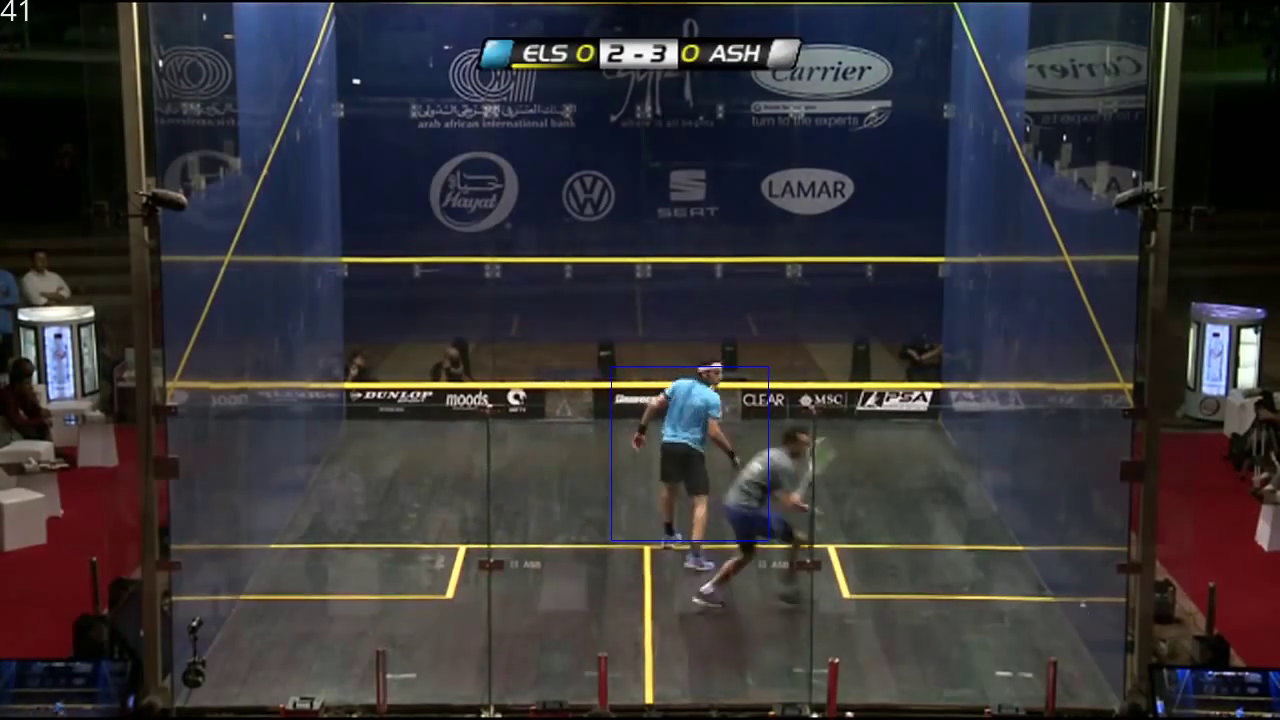
\includegraphics[width=\columnwidth]{./Slike/squash-1-kcf-example.png}
      \caption{41. slika posnetka \cite{squashtv2014squash} s KCF sledilnikom.}
      \label{fig:squash-1-kcf}
    \end{subfigure}
    ~
    \begin{subfigure}[t]{0.45\columnwidth}
      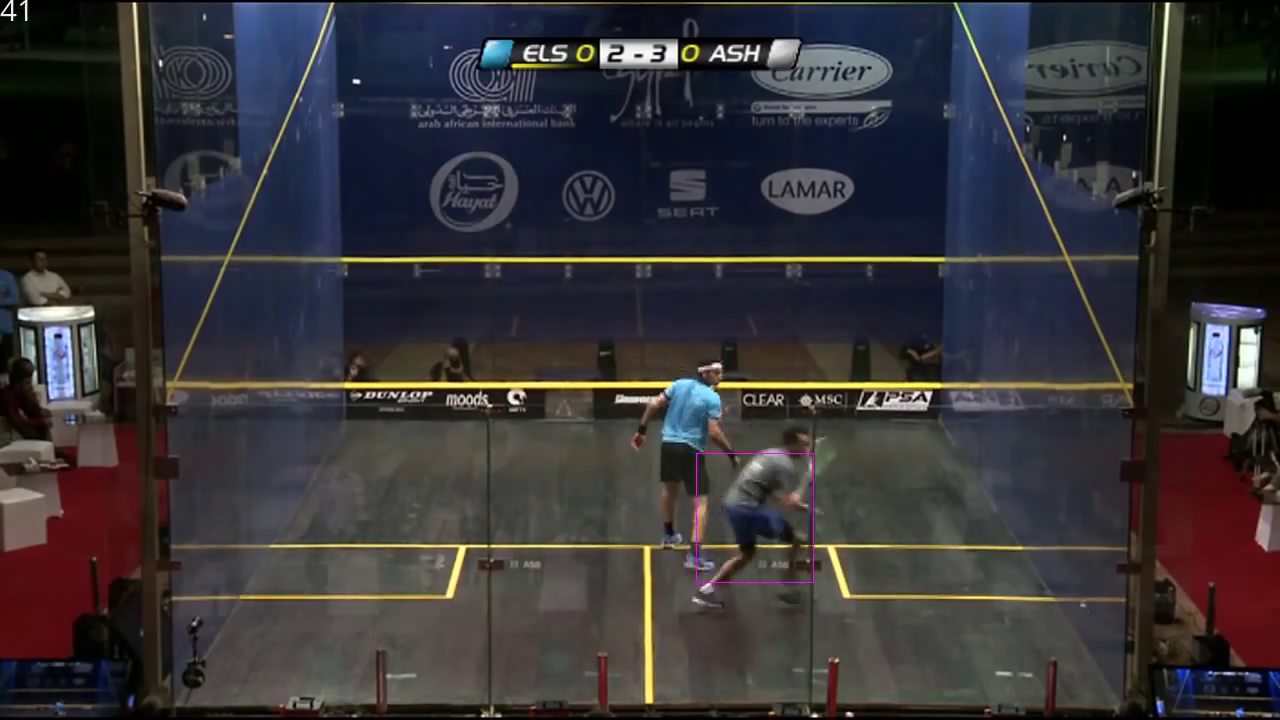
\includegraphics[width=\columnwidth]{./Slike/squash-1-corr-example.png}
      \caption{41. slika posnetka \cite{squashtv2014squash} s CORR sledilnikom.}
      \label{fig:squash-1-corr}
    \end{subfigure}  
\caption[Primer delovanja sledilnikov za squash posnetek]{Primer delovanja sledilnikov za squash posnetek. Gre za identični sliki posnetka, pri čemer smo na sliki \ref{fig:squash-1-kcf} uporabili KCF algoritem, na sliki \ref{fig:squash-1-corr} pa CORR algoritem. Sledilnika sta morala slediti igralcu z modro majico.}
\label{fig:squash-tracker-visual}
\end{figure}


Boljše delovanje KCF je razumljivo, saj prvi testi temeljijo na posnetkih rokometa, drugi pa na squashu, kjer gre za bistveno drugačno igro. Če pogledamo tabelo \ref{tab:region-overlap} ima KCF drugo najboljše povprečje, prav tako pa so si rezultati posameznih posnetkov zelo podobni. 


\subsubsection{Sledilnik za prostorski tok}
Na podlagi pogojev iz poglavja \ref{sec:pogoji-sledilnikov} smo za merilno metodo s prostorskim tokom našli le DS-KCF sledilnik avtorja Hannuna et. al \cite{hannuna2016ds}. 





\subsection{Kalmanov filter}
Za prostor stanj smo izbrali stanje hitrosti $v$ in pospeška $a$ \eqref{eq:stanje}. 

\begin{equation}
\vec{x}(k) = \begin{bmatrix}
					v(k) & a(k)
				\end{bmatrix}^\top 
                \label{eq:stanje}
\end{equation}

Matrika prehajanja stanj je določena z enačbo \eqref{eq:a}.

\begin{equation}
\vec{A} = \begin{bmatrix}
				1 & 1 \\
                0 & 1
			\end{bmatrix} 
            \label{eq:a}
\end{equation}

Za matriko vhodnih stanj $G$ smo izbrali \eqref{eq:g}, s katero modeliramo neznane vhodne parametre hitrosti $v_n$ in pospeška $a_n$ v vektorju $u$ \eqref{eq:u}. 

\begin{equation}
\vec{G} = \begin{bmatrix}
				1 & 0
			\end{bmatrix}^\top 
            \label{eq:g}
\end{equation}

\begin{equation}
\vec{u}(k) = \begin{bmatrix}
					v_{n}(k) & a_n(k)
				\end{bmatrix}^\top 
                \label{eq:u}
\end{equation}


Merilna matrika je predstavljena z enačbo \eqref{eq:h}
\begin{equation}
\vec{H} = \begin{bmatrix}
				1 & 0
			\end{bmatrix}^\top 
            \label{eq:h}
\end{equation}

Za začetno hitrost in pospešek smo izbrali vrednost $0$, ker se naši testi večinoma začnejo v mirovanju. 

Variance šuma modela gibanja, merilnega modela in konvaričane matrike stanja smo določili z uporabo mrežnega iskanja, ki je opisan v poglavju \ref{sec:optimizacija-svm-parametrov}. Pri tem smo uporabili labele učnih vzorcev vseh testov 1. sklopa eksperimentov za referenco, njihove pošumljene ocene pa za meritev. Varianca šuma merilnega modela je tako znašala $\sigma_\vec{z}^2 = 0.04$, varianca šuma modela gibanja pa $\sigma_\vec{x}^2 = 456.13$. Za kovariančno matriko predikcije smo uporabili varianco $\sigma_\vec{P}^2 = 456.13$. Kovariančno matriko modela gibanja smo določili po enačbi \eqref{eq:Q}, kovariančna matrika merilnega modela je bila določena z enačbo \eqref{eq:R} in začetna vrednost kovariančne matrike stanja z \eqref{eq:P}.

\begin{equation}
\vec{Q} = \vec{G} \vec{G}^\top \sigma_\vec{x}^2
\label{eq:Q}
\end{equation}

\begin{equation}
\vec{R} = \sigma_\vec{z}^2
\label{eq:R}
\end{equation}

\begin{equation}
\vec{P}(0) = \begin{bmatrix}
1 & 0 \\
0 & 1
\end{bmatrix} \sigma_\vec{P}^2
\label{eq:P}
\end{equation}





\subsubsection{Optimizacija Gaussovega jedra}
Pri optimizaciji Gaussovega jedra smo določili optimalni standardni odklon $\sigma$ z uporabo dveh metrik, in sicer: koren srednje kvadratične napake (RMSE) in razmerje med signalom in šumom (SNR). Pri RMSE metriki smo določili napako med učnimi vzorci in njihovo predikcijo. Pri SNR metriki smo za signal uporabili referenčne učne vzorce. Za šum smo uporabili rezidualni ali preostali šum. Tega smo dobili z odštevanjem filtriranih vzorcev od referenčnih. SNR metrika tako določa uspešnost izločevanja šuma, RMSE metrika pa pravilnost določevanja kateri podatki spadajo v signal in kateri v šum.


Teste smo izvajali na vseh eksperimentih 1. sklopa, pri čemer smo uporabili $\nu$-RBF jedro s \SI{50}{\%} podpornih vektorjev. Za filtriranje pri mrežnem iskanju smo izbrali najmanjši filter s $\sigma = 1$. Testirali smo naslednje standardne odklone Gaussovega filtra: $1, 3, 5, 11, 21, 31$ in $51$. 

Rezultati povrprečnih vrednosti uporabljenih metrik so vidni v tabeli \ref{tab:gauss}. Za pravilno razlago rezultatov, moramo upoštevati tudi grafe metrik posameznih eksperimentov, ki so prikazani na slikah \ref{fig:sigma1-5}, \ref{fig:sigma-rmse5-21} in \ref{fig:sigma21-51}. 



\begin{table}[htb]
	\centering
    \begin{tabular}{S[table-format=2.0] S[table-format=2.3] S[table-format=2.3]}
    \toprule
    \thead{$\sigma$} & \thead{RMSE} & \thead{SNR [dB]}  \\
    \midrule%nSV
    1 & \boldentry{2.3}{8.614} & 24.278 \\
    3 & 11.236 & 25.470 \\
    \boldentry{2.0}{5} & 11.596 & 25.746 \\
    11 & 11.783 & 25.746 \\
    21 & 11.842 & 25.975 \\
    31 & 11.871 & 26.194 \\
    51 & 11.907 & \boldentry{2.3}{26.306} \\
    \bottomrule
    \end{tabular}
    \caption[Povprečne vrednosti RMSE in SNR metrik pri optimizaciji parametra $\sigma$ Gaussovega filtra]{Povprečne vrednosti RMSE in SNR metrik pri optimizaciji parametra $\sigma$ Gaussovega filtra. Najmanjši standardni odklon ima najmanjšo napako, vendar je tudi filtriranje majhno. Pri $\sigma=3$ in $\sigma=5$ so še opazne razlike pri filriranju. Za višje vrednosti ni več opazne razlike, vendar pa se napaka povečuje. $\sigma=5$ je tako optimalna vrednosti parametra.}
    \label{tab:gauss}
\end{table}

Najmanjšo napako dobimo, če uporabimo $\sigma=1$, vendar pa imamo pri tem najmanjše filtriranje, zato so rezultati še vedno lahko zelo šumni. Z višanjem parametra filtra, se napaka po metriki RMSE povečuje, vendar ima večji vpliv razmerje SNR, saj je predstavljeno v logaritemski skali. 

\begin{figure}[htb]
\centering
\begin{subfigure}[t]{0.45\columnwidth}
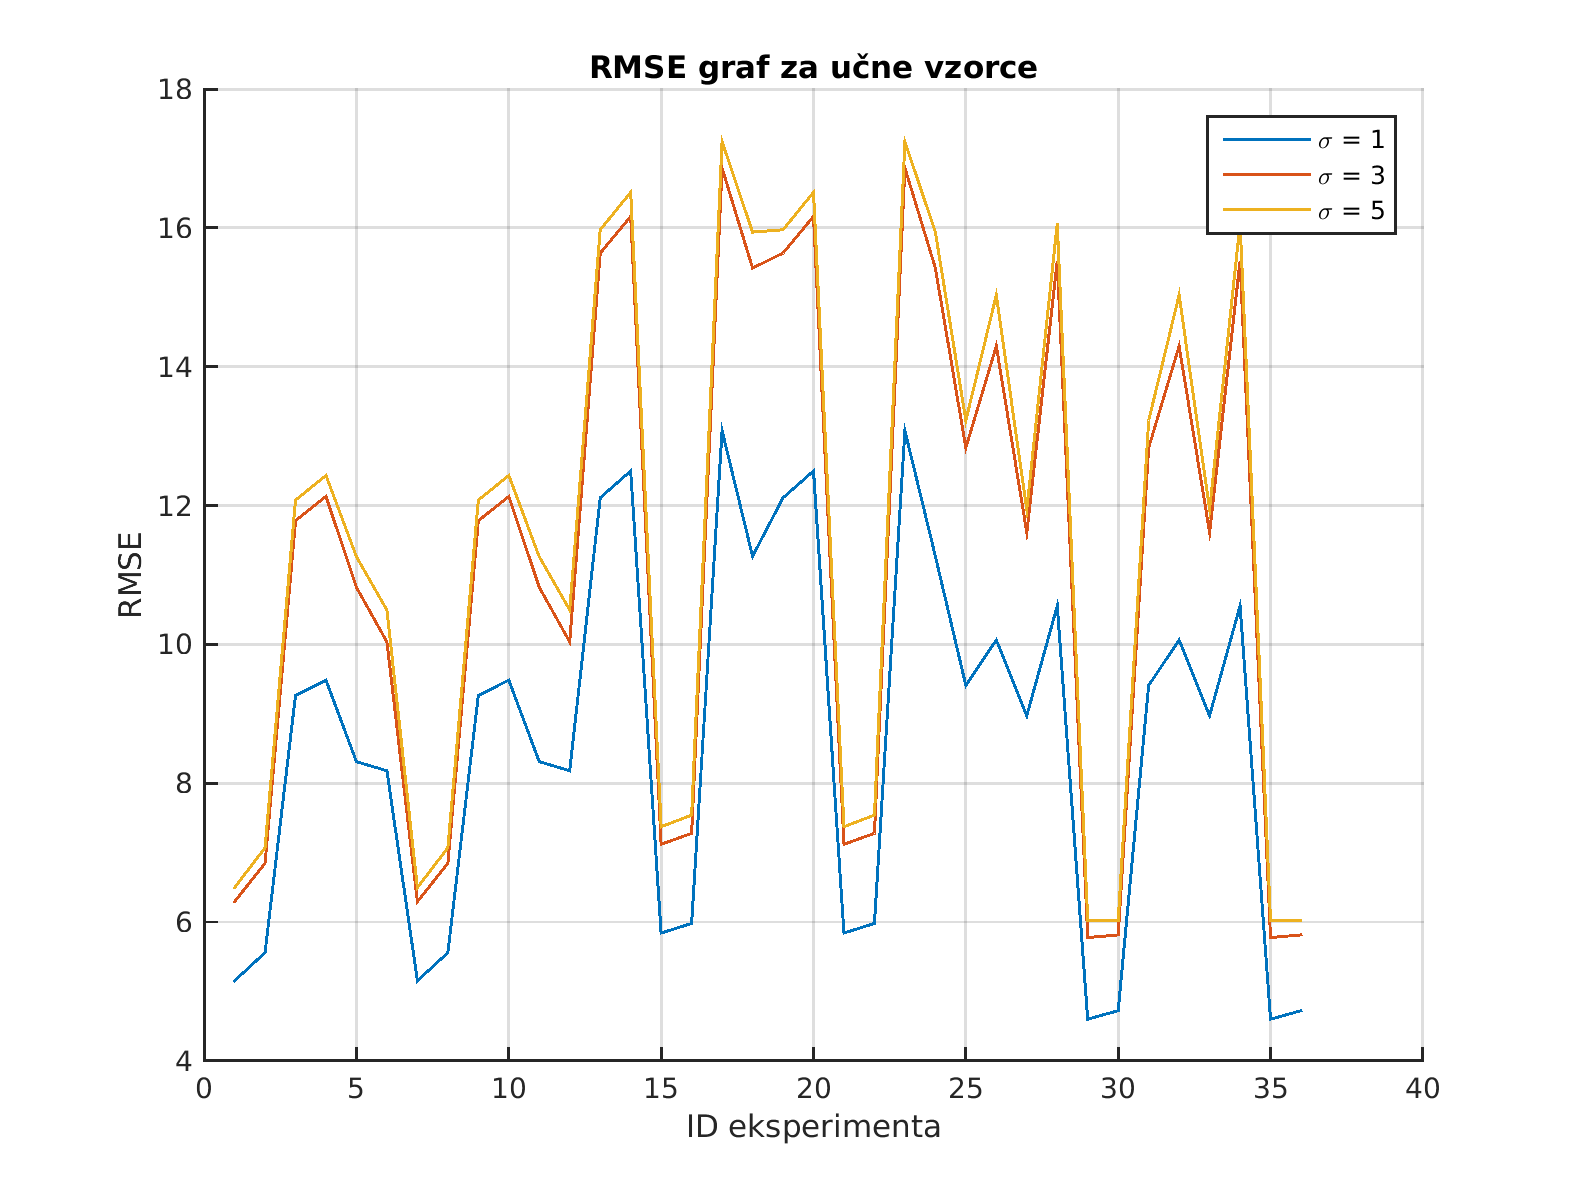
\includegraphics[width=\columnwidth]{./Slike/sigma-rmse1-5.png}
\caption{Graf RMSE  učnih vzorcev }
\label{fig:sigma-rmse1-5}
\end{subfigure}
~
\begin{subfigure}[t]{0.45\columnwidth}
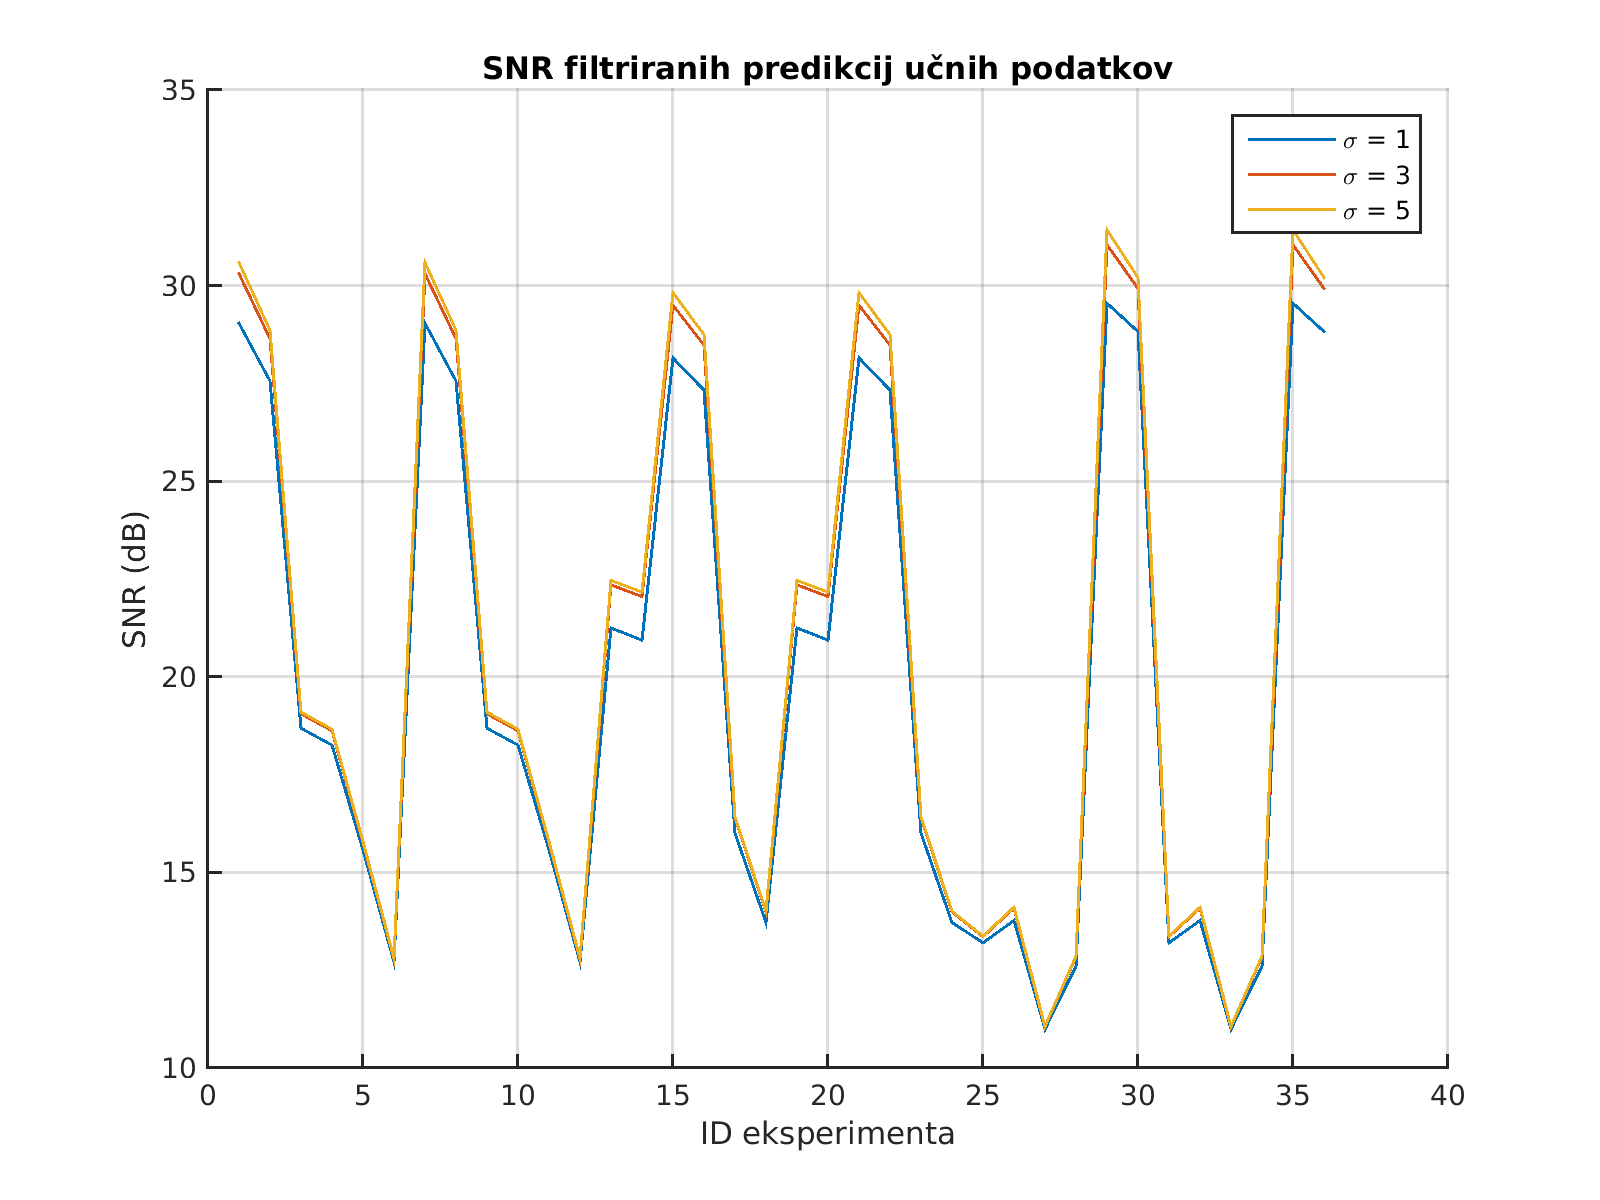
\includegraphics[width=\columnwidth]{./Slike/sigma-snr1-5.png}
\caption{Graf SNR  učnih vzorcev}
\label{fig:sigma-snr1-5}
\end{subfigure}
\caption{Grafa RMSE in SNR učnih vzorcev za \mbox{$\sigma \in [1,5]$}}
\label{fig:sigma1-5}
\end{figure}

Čeprav pri uporabi $\sigma=51$ dobimo največje filtriranje šuma, lahko na slikah grafov opazimo, da se obe metriki bistveno ne razlikujeta za vrednosti parametra na intervalu $[5,51]$. Kljub dobremu filtriranju želimo zagotoviti čim manjšo napako med referenčnim signalom in predikcijo, zato je logična izbira čim manjši standardni odklon. Ker so na sliki \ref{fig:sigma1-5} med $\sigma=3$ in $\sigma=5$ še opazne razlike, lahko zaključimo, da je $\sigma=5$ optimalna izbira parametra za naš problem. 


\begin{figure}[htb]
\centering
\begin{subfigure}[t]{0.45\columnwidth}
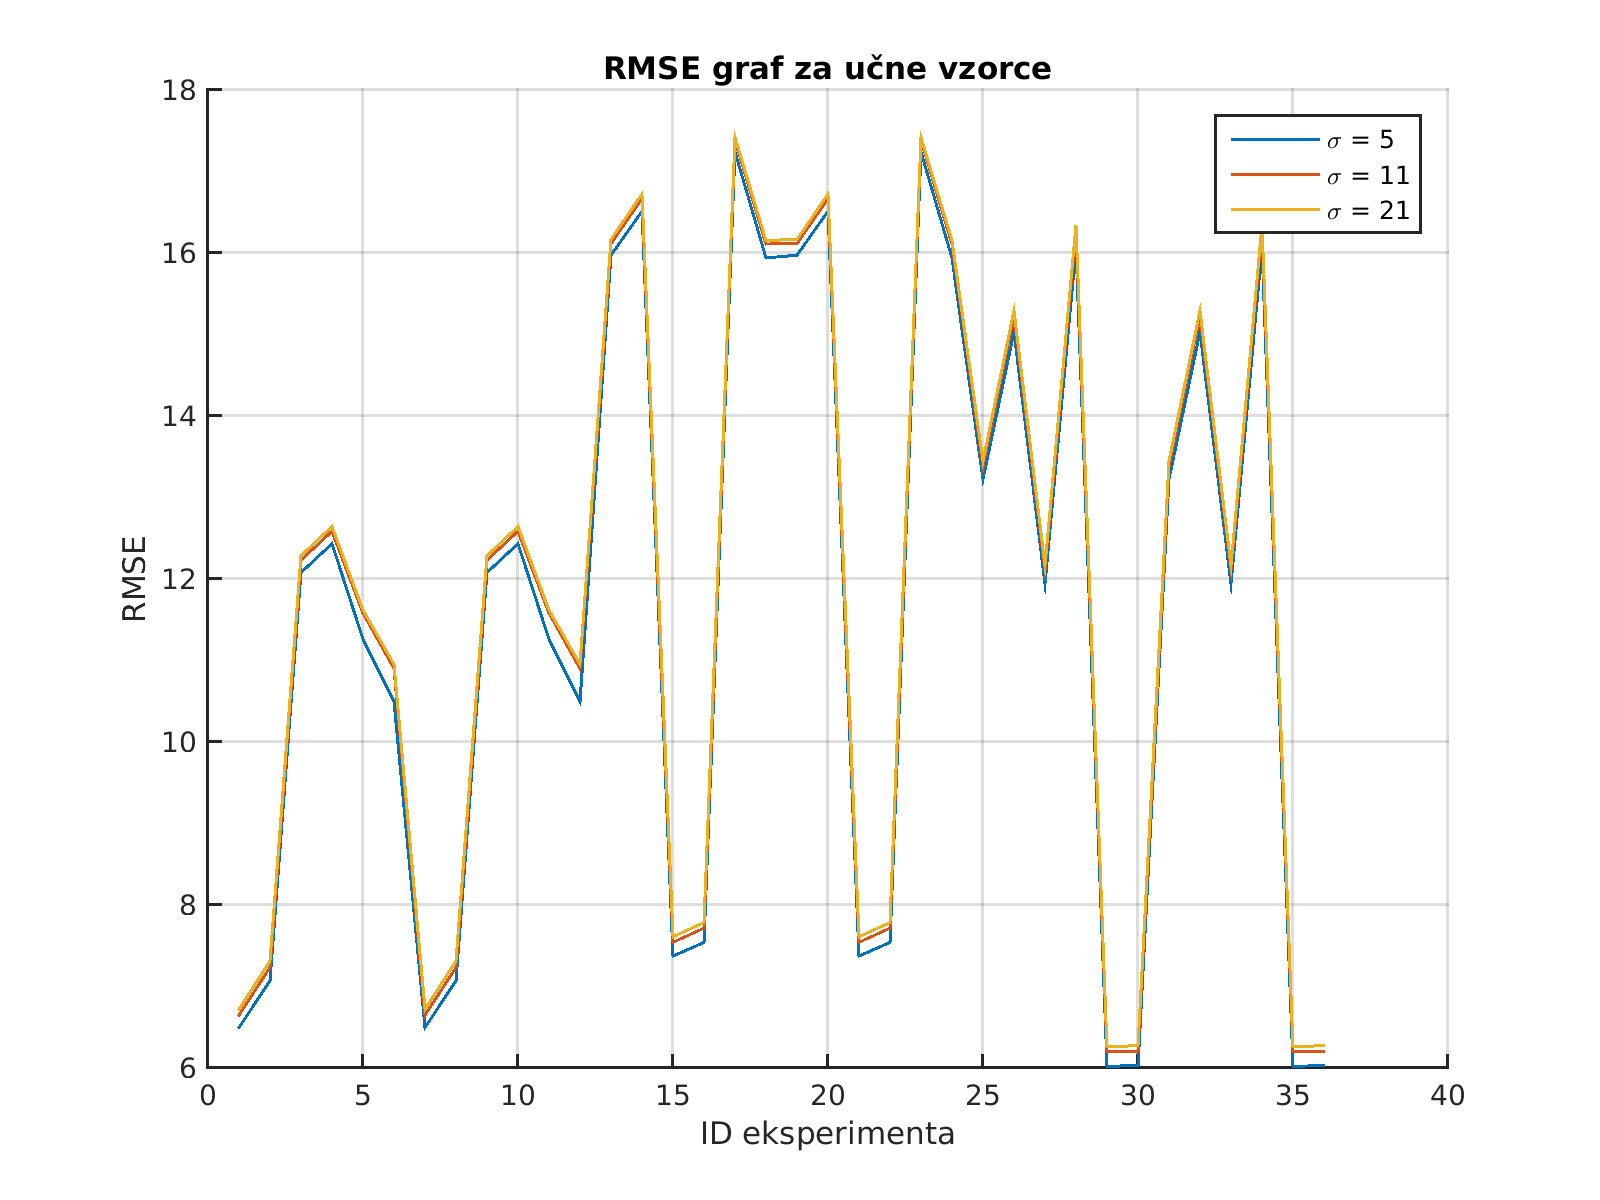
\includegraphics[width=\columnwidth]{./Slike/sigma-rmse5-21.png}
\caption{Graf RMSE  učnih vzorcev}
\label{fig:sigma-rmse5-21}
\end{subfigure}
~
\begin{subfigure}[t]{0.45\columnwidth}
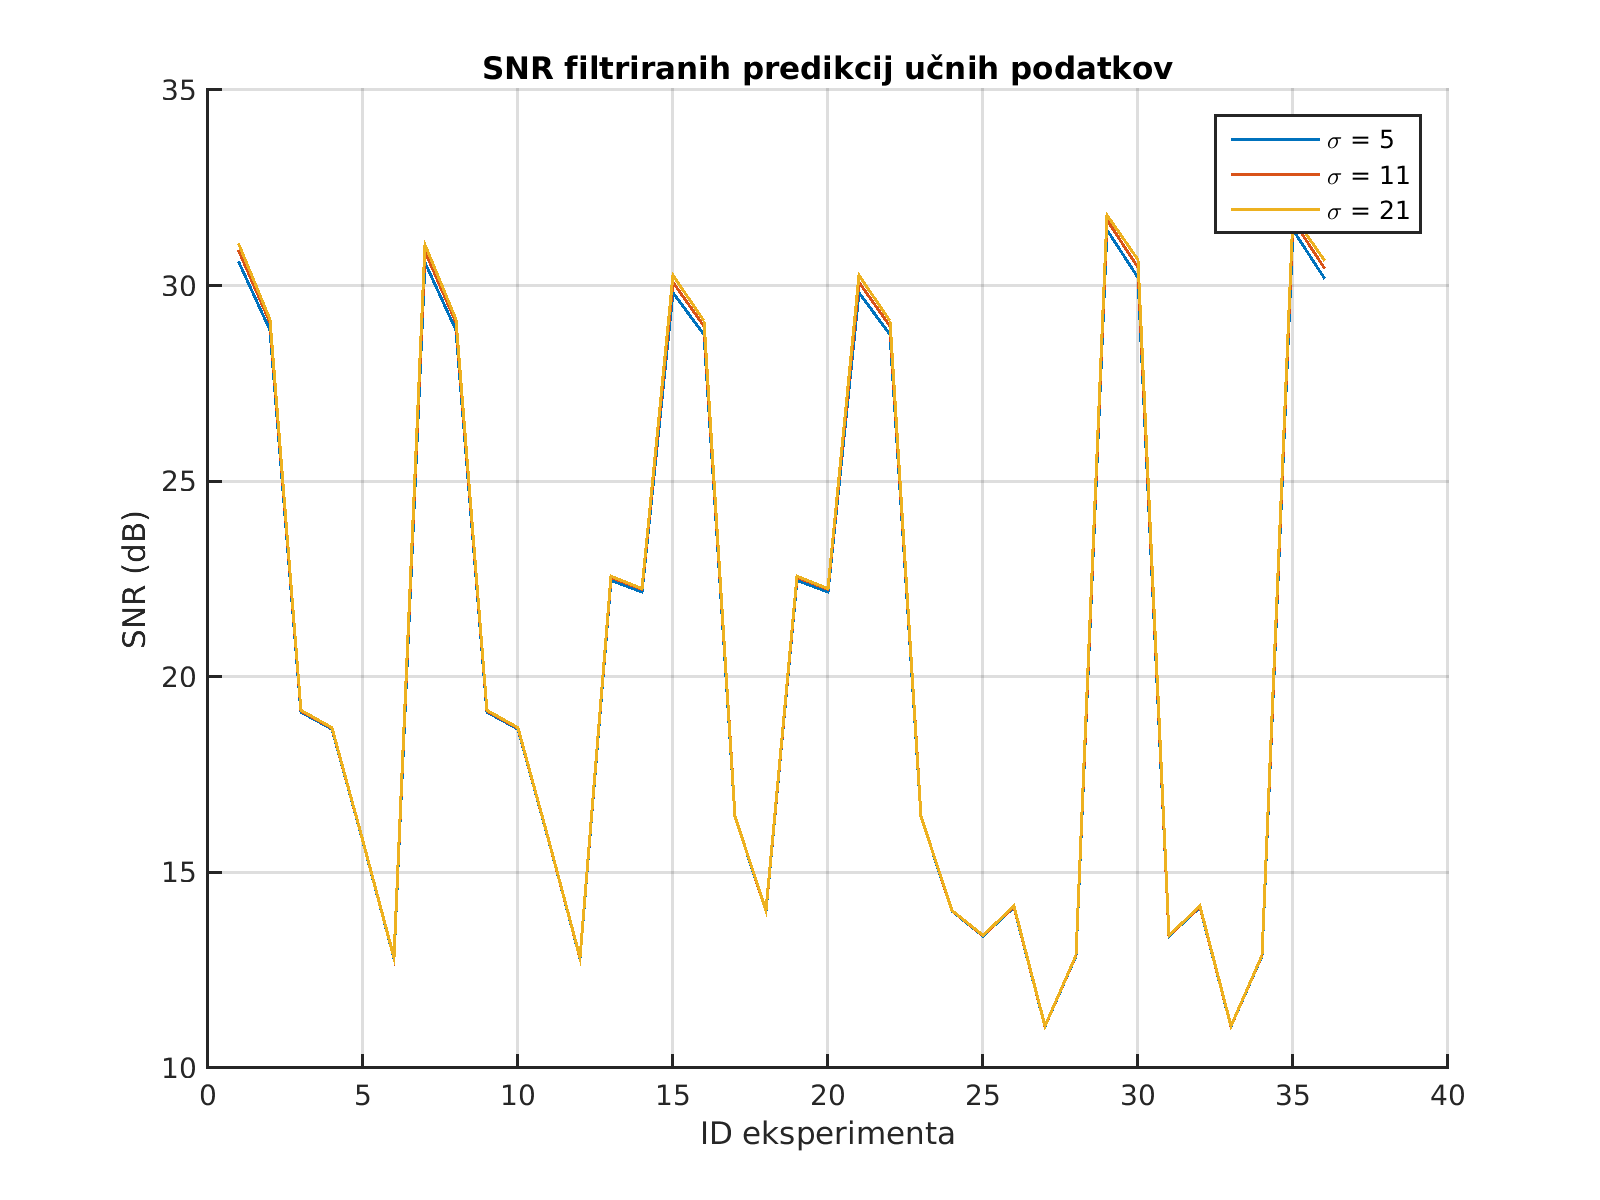
\includegraphics[width=\columnwidth]{./Slike/sigma-snr5-21.png}
\caption{Graf SNR  učnih vzorcev}
\label{fig:sigma-snr5-21}
\end{subfigure}
\caption{Grafa RMSE in SNR učnih vzorcev za \mbox{$\sigma \in [5,21]$}}
\label{fig:sigma5-21}
\end{figure}



\begin{figure}[htb]
\centering
\begin{subfigure}[t]{0.45\columnwidth}
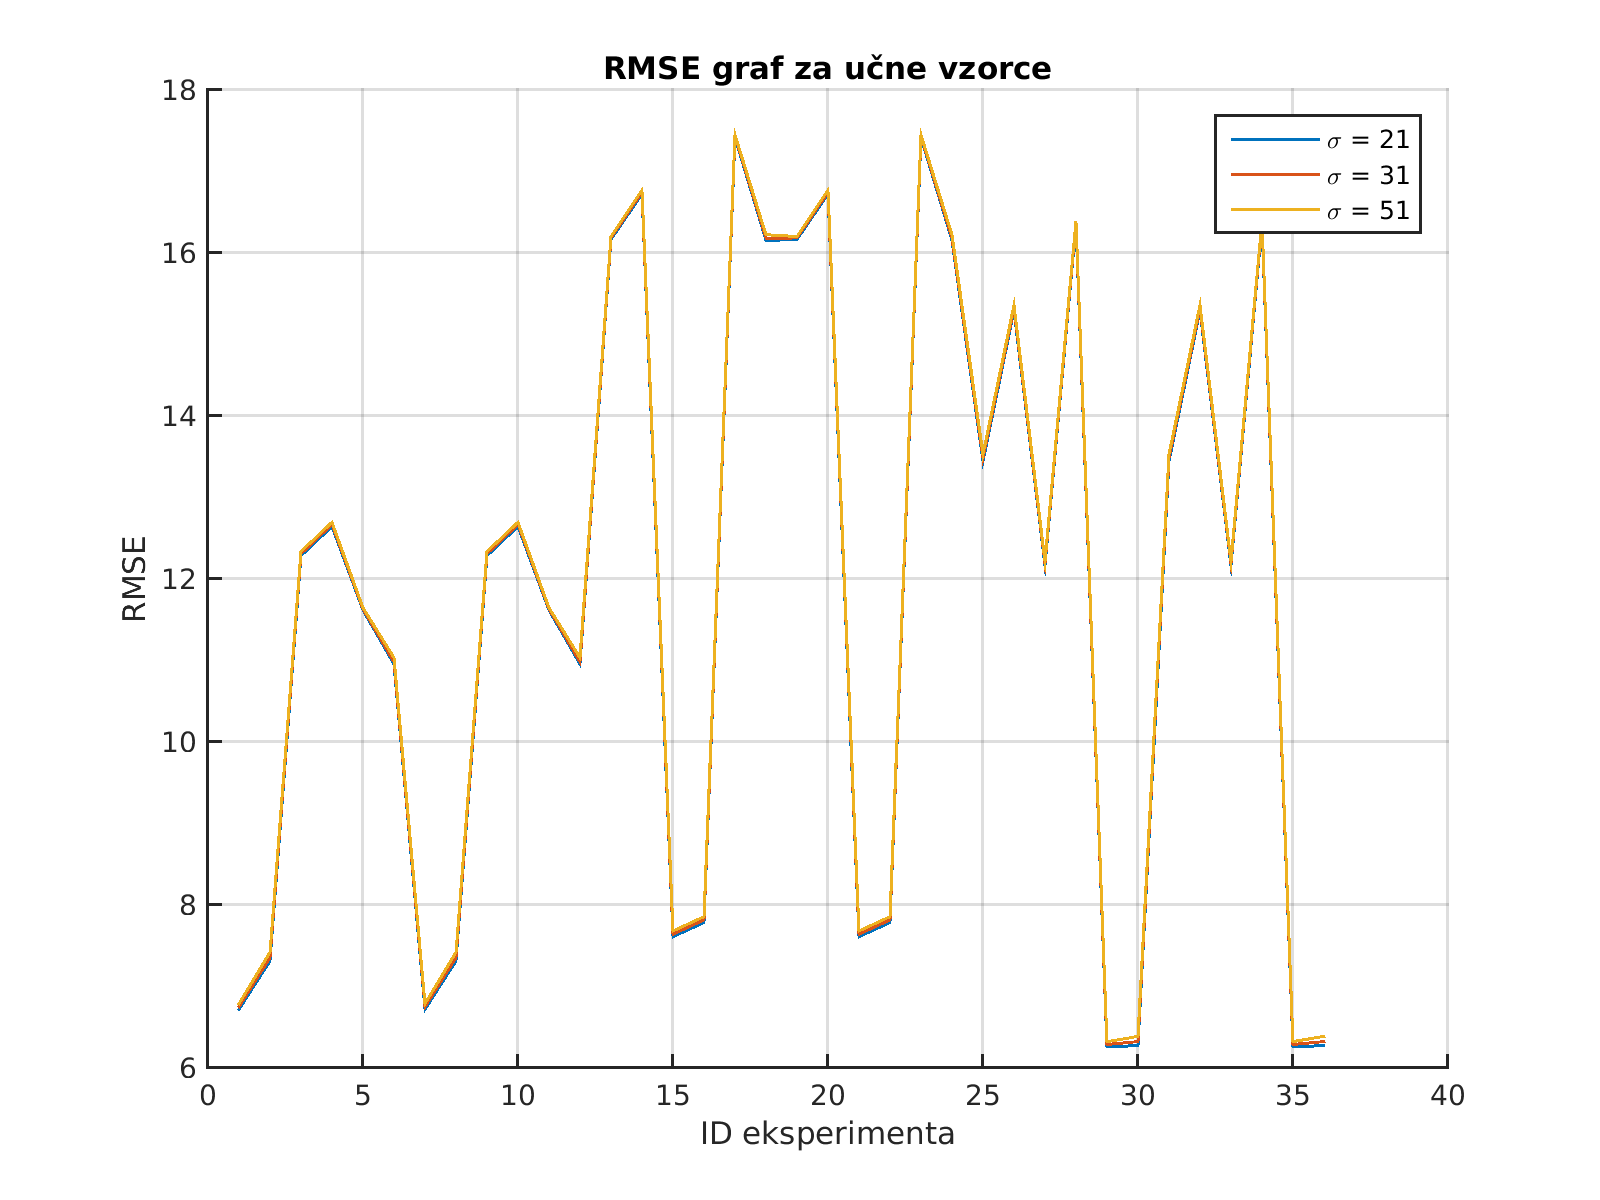
\includegraphics[width=\columnwidth]{./Slike/sigma-rmse21-51.png}
\caption{Graf RMSE učnih vzorcev}
\label{fig:sigma-rmse21-51}
\end{subfigure}
~
\begin{subfigure}[t]{0.45\columnwidth}
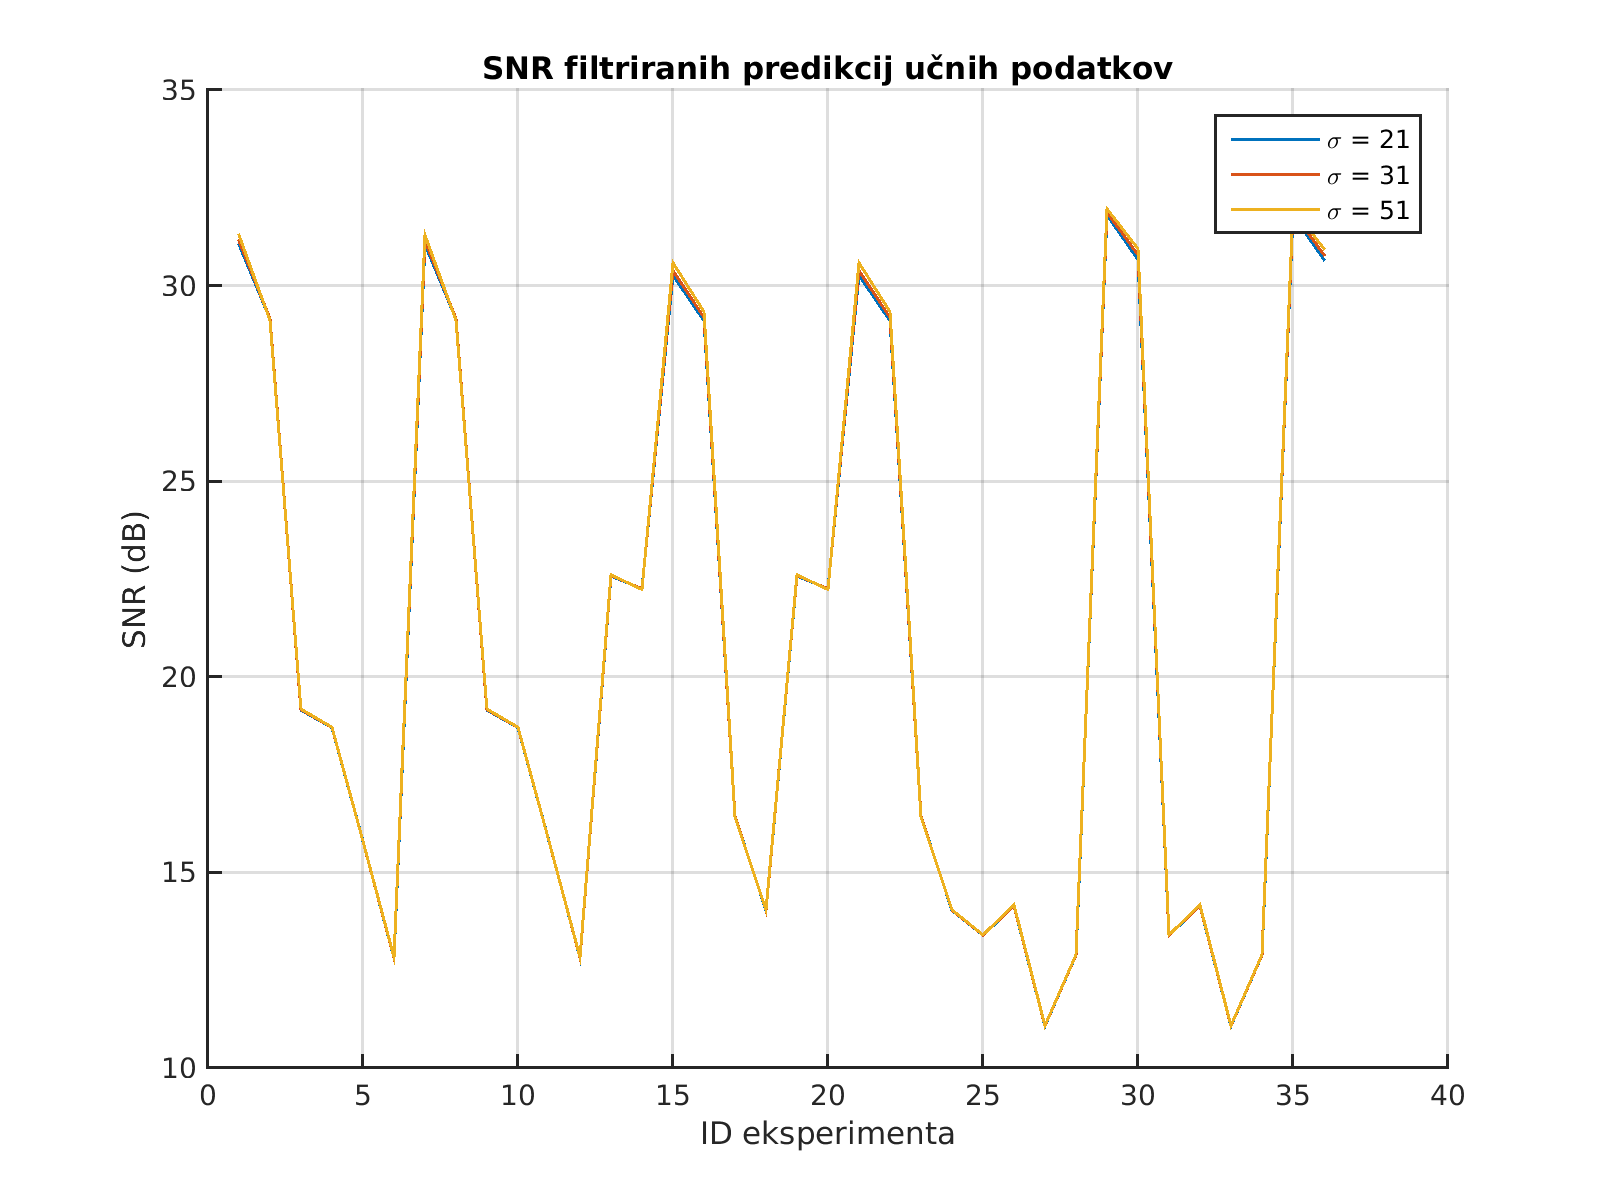
\includegraphics[width=\columnwidth]{./Slike/sigma-snr21-51.png}
\caption{Graf SNR  učnih vzorcev}
\label{fig:sigma-snr21-51}
\end{subfigure}
\caption{Grafa RMSE in SNR učnih vzorcev za \mbox{$\sigma \in [21,51]$}}
\label{fig:sigma21-51}
\end{figure}



\subsection{Implementacija Gaussovega filtra}
Gaussovo jedro smo implementirali po enačbi \eqref{eq:gauss} in ga nato še normirali. Za filtriranje podatkov smo uporabili Matlabovo funkcijo \texttt{filtfilt}, ki je primerna za hitro računanje s filtri z ničelno fazo, saj uporablja tehniko dvosmernega filtriranja.




\subsection{Projektivna transformacija preliminarnih testov}
Projektivno transformacijo smo izvedli s pomočjo matlabovih funkcij \texttt{fitgeotrans} in \texttt{imwarp}. Za vhodne točke smo izbrali robove posamezne slike zaporedja. Za izhodne točke smo izbrali vrednosti v tabeli \ref{tab:projective}, pri čemer so $h$ dolžina slike $w$ širina slike ter $x$ in $y$ slikovni koordinati.

\begin{table}[htb]
\centering
\begin{tabular}{l S[table-format=1.3] S[table-format=1.3] }
	\toprule
	\thead{Točka} & \thead{$x~[\times w]$} & \thead{$y~[\times h]$} \\
    \midrule
	$P_0$ & 0 & 0.25 \\
    $P_1$ & 1 & 0 \\
    $P_2$ & 0.125 & 0.75 \\
    $P_3$ & 0.875 & 0.875 \\
    \bottomrule
\end{tabular}
\caption{}
\label{tab:projective}
\end{table}

\subsection{Simulacija vibracij kamere}
Kadar uporabljamo ročne kamere, pogosto pride do tresenja. Vibracije smo simulirali z majhnimi naključnimi premiki in rotacijo posameznih slik iz video zaporedja. Vsako sliko smo transformirali z Evklidsko transformacijo. Pri tem smo translacijo omejili na \SI{4}{\%} velikosti slike. Rotacija je bila omejena na \SI{0.13}{rad}. 

Translacijo in rotacijo smo filtrirali še s Kalmanovim filtrom, tako da smo dobili bolj realistično simulacijo. Za Kalmanov filter smo uporabili enak model, kot je predstavljen v poglavju \ref{sec:kalmanov-filter}. Začetne variance filtra smo določili empirično tako, da smo dobili čimbolj realistične rezultate. Varianca šuma merilnega modela je znašala $\sigma_\vec{z}^2=1024$, variancal šuma modela gibanja pa $\sigma_\vec{x}^2=2$. Za kovariančno matriko predikcije smo uporabili varianco $\sigma_\vec{P}^2=2$.


\subsection{Združevanje slik iz dveh Kinect kamer}
Zaradi ozkega vidnega polja Kinect kamer smo za pokritje celotne širine igrišča potrebovali dve kameri. Zaporedja slik smo pred nadaljno obdelavo morali združiti v eno zaporedje glede na opazovanega igralca.

Zajem iz posameznih kamer ni bil sinhroniziran, zato smo pred združevanjem sinhronizirali posnetka tako, da smo izbrali slike iz posameznega zaporedja z najbolj podobnimi časovnimi žigi. 

\subsubsection{Združevanje z značilkami}
Časovno sinhronizirana zaporedja slik, smo najprej poskušali združiti z metodo panoramskega šivanja slik z uporabo značilk, kot je opisano v delu \cite{brown2007automatic}. Tu smo namesto SIFT značilk uporabili SURF značilke. Združevanje s značilkami se ni obneslo, zato smo to metodo opustili. Primer neuspelega poskusa je prikazan na sliki \ref{fig:zdruzevanje-znacilke}.

\begin{figure}[htb]
\centering
\begin{subfigure}[t]{0.45\columnwidth}
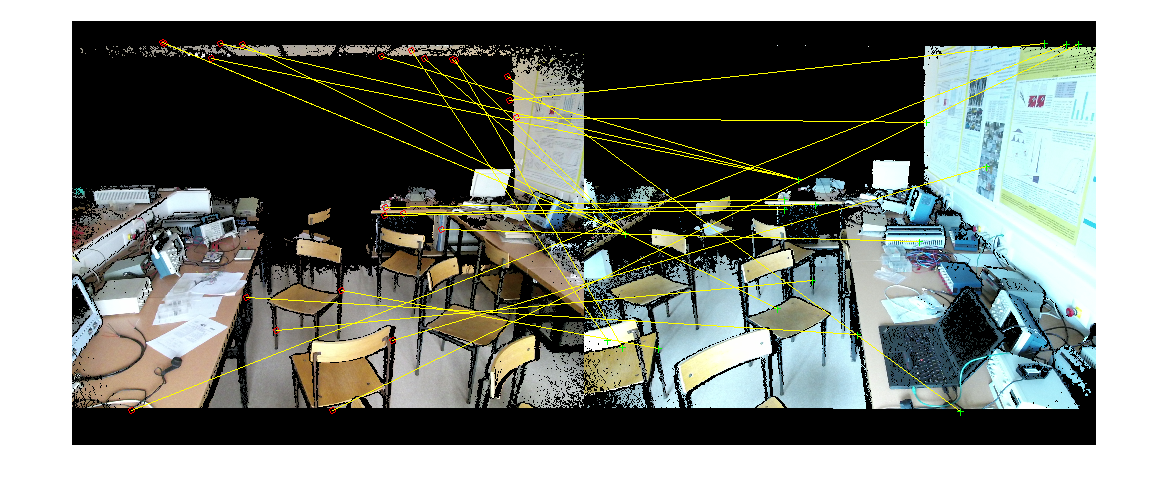
\includegraphics[width=\columnwidth]{./Slike/matched-features.png}
\caption{Ujemajoče SURF značilke}
\label{fig:zdruzevanje-surf}
\end{subfigure}
~
\begin{subfigure}[t]{0.45\columnwidth}
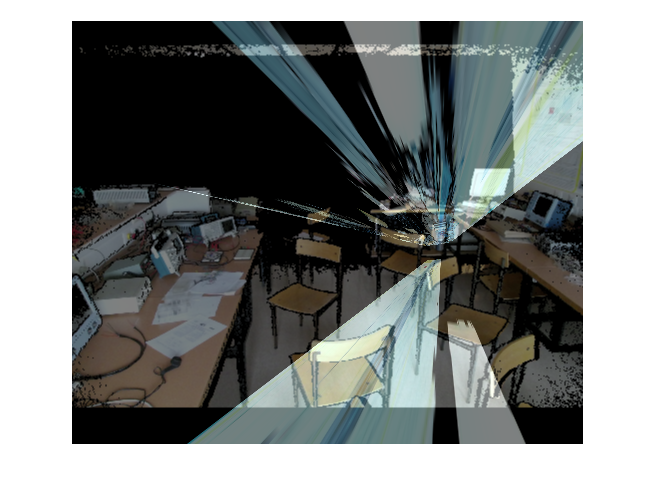
\includegraphics[width=\columnwidth]{./Slike/features-calibration-result.png}
\caption{Rezultat združevanja z značilkami}
\label{fig:zdruzevanje-result}
\end{subfigure}
\caption{Primer neuspelega poskusa združevanja slik iz dveh Kinect kamer s SURF značilkami.}
\label{fig:zdruzevanje-znacilke}
\end{figure}

\subsubsection{Združevanje s kontrolnimi točkami}
Zaporedja slik smo poskušali združiti z ročnim določevanjem kontrolnih točk. Rezultat je bil boljši od združevanja z značilkami, vendar še vedno slab, zato smo tudi to metodo opustili. Primer neuspelega poskusa je prikazan na sliki \ref{fig:zdruzevanje-cp}.

\begin{figure}[htb]
\centering
\begin{subfigure}[t]{0.45\columnwidth}
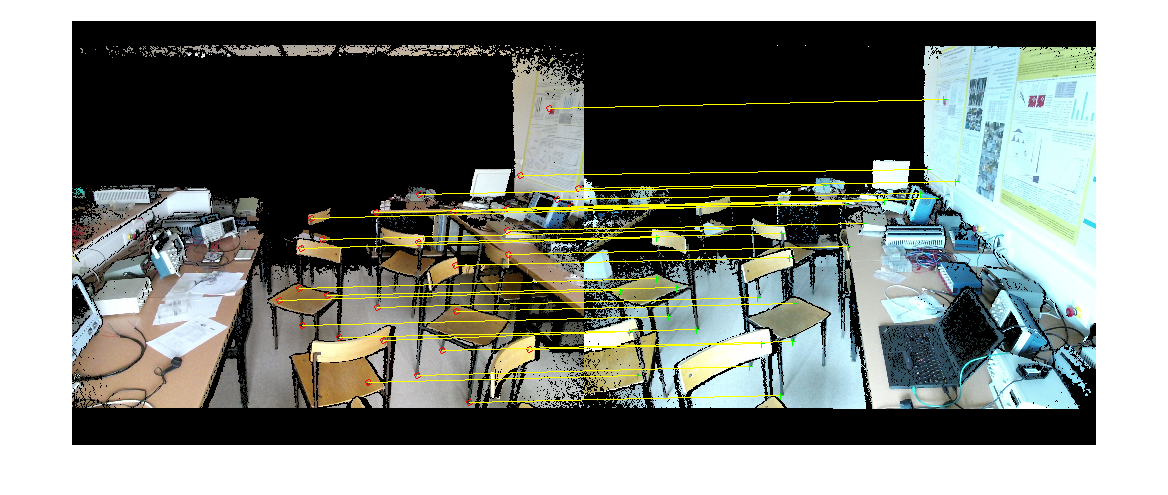
\includegraphics[width=\columnwidth]{./Slike/matched-points.png}
\caption{Ujemajoče kontrolne točke}
\label{fig:zdruzevanje-ujemajoce-cp}
\end{subfigure}
~
\begin{subfigure}[t]{0.45\columnwidth}
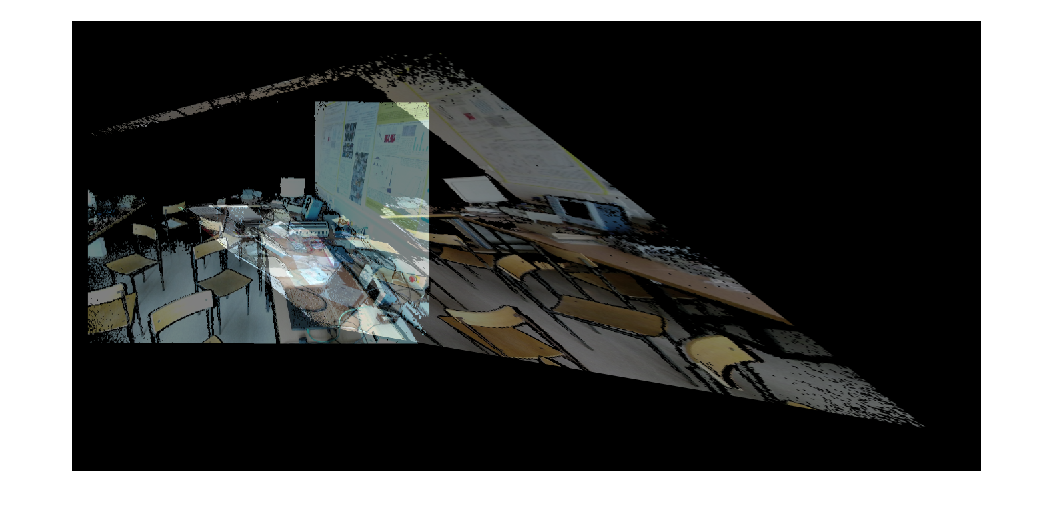
\includegraphics[width=\columnwidth]{./Slike/points-calibration-result.png}
\caption{Rezultat združevanja s kontrolnimi točkami}
\label{fig:zdruzevanje-result-cp}
\end{subfigure}
\caption{Primer neuspelega poskusa združevanja slik iz dveh Kinect kamer s kontolnimi točkami}
\label{fig:zdruzevanje-cp}
\end{figure}


\subsubsection{Prilagojeno združevanje}
Zaradi nezadovoljivih rezultatov klasičnih metod združevanja stereo slik, smo razvili metodo, ki je prilagojena za Kinect kamere. Iz kamer smo pridobili intrinzične parametre infra-redečega (IR) senzora, in sicer: slikovni koordinati goriščne razdalje $f_u$ in $f_v$ ter slikovni koordinati optičnega središča slike (ang. principal point) $c_u$ in $c_v$. Intrinsične parametre smo uporabili za določitev intrizične matrike $\vec{M}_{int}$ po enačbi \eqref{eq:intrinsic}.


Ker pravih ekstrinsičnih parametrov kamer nismo poznali, smo jih le ocenili z metodo določevanja sečišča vidnih polj obeh kamer. Sečišče je prikazano kot rdeča linija na sliki \ref{fig:zdruzevanje}. S to metodo smo določili translacijski vektor $\vec{t} = \left [ t_x~ t_y~ t_z \right]^\top$ in rotacijsko matriko $\vec{R}$ 

Ekstrinsične parametre smo določili s pomočjo posebnega programa, kjer smo določili centralno linijo med njima -> slika. pa še sledenje z dskcf. Potem smo pa s pomočjo homografije določili metrični center tarče na trenutni kameri on gledali kdaj bo šel čez mejo, pri čemer smo imeli še upragovljeno, da ni preveč skakalo 

z -> forward -> roll $\phi$
-y -> up -> yaw $\psi$
-x -> left -> pitch $\theta$



enačba intrinsične matrike enačba ekstrinsične matrike, enačba homografije enačba transformacije v metrični center iz lokalnega, vsi parametri-> velikost praga.

slika
\begin{figure}[htb]
\centering
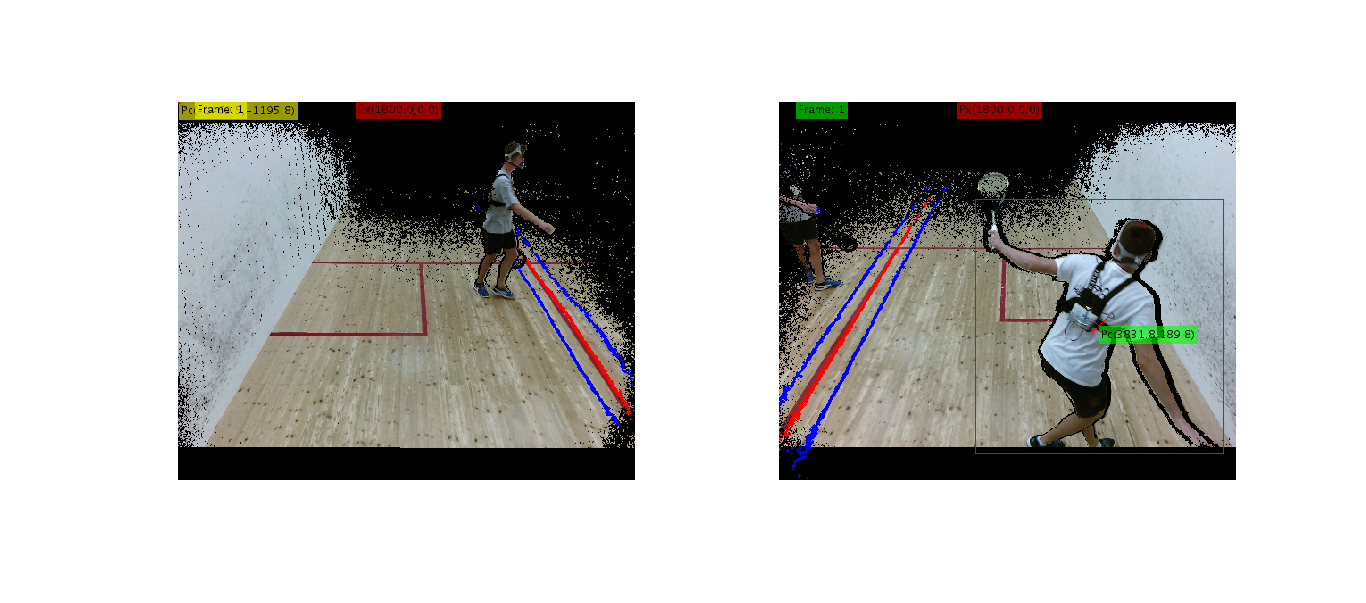
\includegraphics[width=\columnwidth]{./Slike/zdruzevanje-example.png}
\caption{}
\label{fig:zdruzevanje}
\end{figure}











\section{Eksperimenti 1. faze}
a

\subsection{Laboratorijski eksperimenti}
a

\subsection{Terenski eksperimenti}
a

\section{Eksperimenti 2. faze}
a

\subsection{Laboratorijski eksperimenti}
a

\subsection{Terenski eksperimenti}
a

\section{Rezultati}
a

